
%%
%% forked from https://gits-15.sys.kth.se/giampi/kthlatex kthlatex-0.2rc4 on 2020-02-13
%% expanded upon by Gerald Q. Maguire Jr.
%% This template has been adapted by Anders Sjögren to the University
%% Engineering Program in Computer Science at KTH ICT. This adaptation was
%% translation of English headings into Swedish with the addition of Swedish.
%% Many thanks to others who have provided constructive input regarding the template.

% Make it possible to conditionally depend on the TeX engine used
\RequirePackage{ifxetex}
\RequirePackage{ifluatex}
\newif\ifxeorlua
\ifxetex\xeorluatrue\fi
\ifluatex\xeorluatrue\fi

\ifxeorlua
% The following is to ensure that the PDF uses a recent version rather than the typical PDF 1-5
%  This same version of PDF should be set as an option for hyperef

\RequirePackage{expl3}


\ExplSyntaxOn
%pdf_version_gset:n{2.0}
%\pdf_version_gset:n{1.5}

%% Alternatively, if you have a LaTeX newer than June 2022, you can use the following. However, then you have to remove the pdfversion from hyperef. It also breaks hyperxmp. So perhaps it is too early to try using it!
%\DocumentMetadata
%{
%% testphase = phase-I, % tagging without paragraph tagging
% testphase = phase-II % tagging with paragraph tagging and other new stuff.
%pdfversion = 2.0 % pdfversion must be set here.
%}

% Optionally, you can set the uncompress flag to make it easier to examine the PDF
%\pdf_uncompress: % to check the pdf
\ExplSyntaxOff
\else
\RequirePackage{expl3}
\ExplSyntaxOn
%\pdf_version_gset:n{2.0}
\pdf_version_gset:n{1.5}
\ExplSyntaxOff
\fi

%% Define a pair of commands to disable and reenable specific packages - see https://tex.stackexchange.com/questions/39415/unload-a-latex-package
\makeatletter
\newcommand{\disablepackage}[2]{%
  \disable@package@load{#1}{#2}%
}
\newcommand{\reenablepackage}[1]{%
  \reenable@package@load{#1}%
}
\makeatother
%% To avoid the warning: "Package transparent Warning: Loading aborted, because pdfTeX is not running in PDF mode."
\ifxeorlua
\disablepackage{transparent}{}
\fi

\RequirePackage{etoolbox}

%% The template is designed to handle a thesis in English or Swedish
\documentclass[
english,                 % the language of the body of the document: english or swedish       (note this must be in lower case)
bibtex,                  % the bibliographic processor to use: biblatex or bibtex
%nomenclature,           % add the option nomenclature
%digitaloutput,          % optimize for digital output (this changes the color palette)
%includeExtraAbstracts, % uncomment to allow abstracts in languages beyond English & Swedish
]{kththesis}

% ===== ADD THE FIX ====
\makeatletter
\def\f@nch@orh{\f@nch@olh}
\def\f@nch@elh{\f@nch@erh}
\makeatother
% ===== END OF FIX =====

% ===== SUPPRESS WARNINGS =======
\RequirePackage{silence}
\WarningFilter{fancyhdr}{Command \f@nch@orh}
\WarningFilter{fancyhdr}{Command \f@nch@elh}
\hbadness=10000
\vbadness=10000
% ===== END OF SUPPRESSIONS =====

% if pdflatex \usepackage[utf8]{inputenc}
\usepackage[utf8]{inputenc}

%% Conventions for todo notes:
% Informational
%% \generalExpl{Comments/directions/... in English}
\newcommand*{\generalExpl}[1]{\todo[inline]{#1}}                

% Language-specific information (currently in English or Swedish)
\newcommand*{\engExpl}[1]{\todo[inline, backgroundcolor=kth-lightgreen40]{#1}} %% \engExpl{English descriptions about formatting}
\newcommand*{\sweExpl}[1]{\todo[inline, backgroundcolor=kth-lightblue40]{#1}}  %% % \sweExpl{Text på svenska}

% warnings
\newcommand*{\warningExpl}[1]{\todo[inline, backgroundcolor=kth-lightred40]{#1}} %% \warningExpl{warnings}

% Uncomment to hide specific comments, to hide **all** ToDos add `final` to
% document class
% \renewcommand\warningExpl[1]{}
% \renewcommand\generalExpl[1]{}
% \renewcommand\engExpl[1]{}
% For example uncommenting the following line hides the Swedish language explanations
% \renewcommand\sweExpl[1]{}


% \usepackage[style=numeric,sorting=none,backend=biber]{biblatex}
\iftoggle{biblatex}{
    %\usepackage[language=english,bibstyle=authoryear,citestyle=authoryear, maxbibnames=99]{biblatex}
    % Alternatively you might use another style, such as IEEE and use citestyle=numeric-comp  to put multiple citations in a single pair of square brackets
    \usepackage[style=ieee,citestyle=numeric-comp]{biblatex}
    \addbibresource{references.bib}
    %\DeclareLanguageMapping{norsk}{norwegian}
}{
    % The line(s) below are for BibTeX
    \bibliographystyle{bibstyle/myIEEEtran}
    %\bibliographystyle{apalike}
}


% include a variety of packages that are useful
\input{lib/includes}
\input{lib/kthcolors}

%\glsdisablehyper
%\makeglossaries
%\makenoidxglossaries
%\input{lib/acronyms}                %load the acronyms file

\input{lib/defines}  % load some additional definitions to make writing more consistent

% The following is needed in conjunction with generating the DiVA data with abstracts and keywords using the scontents package and a modified listings environment
%\usepackage{listings}   %  already included

\makeatletter
\let\verbatimsc\@undefined
\let\endverbatimsc\@undefined
\lst@AddToHook{Init}{\hyphenpenalty=50\relax}
\makeatother


\lstnewenvironment{verbatimsc}
    {
    \lstset{%
        basicstyle=\ttfamily\tiny,
        backgroundcolor=\color{white},
        %basicstyle=\tiny,
        %columns=fullflexible,
        columns=[l]fixed,
        language=[LaTeX]TeX,
        %numbers=left,
        %numberstyle=\tiny\color{gray},
        keywordstyle=\color{red},
        breaklines=true,                 % sets automatic line breaking
        breakatwhitespace=true,          % sets if automatic breaks should only happen at whitespace
        %keepspaces=false,
        breakindent=0em,
        %fancyvrb=true,
        frame=none,                     % turn off any box
        postbreak={}                    % turn off any hook arrow for continuation lines
    }
}{}

%% Add some more keywords to bring out the structure more
\lstdefinestyle{[LaTeX]TeX}{
morekeywords={begin, todo, textbf, textit, texttt}
}

%% definition of new command for bytefield package
\newcommand{\colorbitbox}[3]{%
	\rlap{\bitbox{#2}{\color{#1}\rule{\width}{\height}}}%
	\bitbox{#2}{#3}}




% define a left aligned table cell that is ragged right
\newcolumntype{L}[1]{>{\raggedright\let\newline\\\arraybackslash\hspace{0pt}}p{#1}}

% Because backref is not compatible with biblatex
\iftoggle{biblatex}{
    \usepackage[plainpages=false]{hyperref}
}{
    \usepackage[
    backref=page,
    pagebackref=false,
    plainpages=false,
                            % PDF related options
    unicode=true,           % Unicode encoded PDF strings
    bookmarks=true,         % generate bookmarks in PDF files
    bookmarksopen=false,    % Do not automatically open the bookmarks in the PDF reading program
    pdfpagemode=UseNone,    % None, UseOutlines, UseThumbs, or FullScreen
    destlabel,              % better naming of destinations
    pdfencoding=auto,       % for unicode in 
    ]{hyperref}
   %% Removed use of backref package as it is incompatible with using attachfile
}

\usepackage[all]{hypcap}	%% prevents an issue related to hyperref and caption linking

%% Acronyms
% note that nonumberlist - removes the cross references to the pages where the acronym appears
% note that super will set the descriptions text aligned
% note that nomain - does not produce a main glossary, thus only acronyms will be in the glossary
% note that nopostdot - will prevent there being a period at the end of each entry
\usepackage[acronym, style=super, section=section, nonumberlist, nomain,
nopostdot]{glossaries}
\setlength{\glsdescwidth}{0.75\textwidth}
\usepackage[]{glossaries-extra}
\ifinswedish
    %\usepackage{glossaries-swedish}
\fi

%% For use with the README_notes
% Define a new type of glossary so that the acronyms defined in the README_notes document can be distinct from those in the thesis template
% the tlg, tld, and dn will be the file extensions used for this glossary
\newglossary[tlg]{readme}{tld}{tdn}{README acronyms}


\input{lib/includes-after-hyperref}

%\glsdisablehyper
\makeglossaries
%\makenoidxglossaries

% The following bit of ugliness is because of the problems PDFLaTeX has handling a non-breaking hyphen
% unless it is converted to UTF-8 encoding.
% If you do not use such characters in your acronyms, this could be simplified to just include the acronyms file.
\ifxeorlua
\input{lib/acronyms}                %load the acronyms file
\else
\input{lib/acronyms-for-pdflatex}
\fi

% place holders for languages lacking .lbx files
\input{lib/placeHolder_lbx_files}

% insert the configuration information with author(s), examiner, supervisor(s), ...
\input{custom_configuration}

% read in the plain text definitions, if they exist
\IfFileExists{custom_configuration_plaintext.tex}{\input{custom_configuration_plaintext.tex}}{}


% Enter the English and Swedish keywords here for use in the PDF metadata _and_ for later use
% following the respective abstract.
% Try to put the words in the same order in both languages to facilitate matching. For example:
\EnglishKeywords{KeywordA, KeywordB, KeywordC}
\SwedishKeywords{NyckelordA, NyckelordB, NyckelordC}

%%%%% For the oral presentation
%% Add this information once your examiner has scheduled your oral presentation
\presentationDateAndTimeISO{2022-03-15 13:00}
\presentationLanguage{XXX}  % generally: eng or swe
\presentationRoom{via Zoom https://kth-se.zoom.us/j/ddddddddddd}
\presentationAddress{Isafjordsgatan 22 (Kistagången 16)}
\presentationCity{Stockholm}

% When there are multiple opponents, separate their names with '\&'
% Opponent's information
%\opponentsNames{A. B. Normal \& A. X. E. Normalè}
\opponentsNames{XXX}

% It is possible to have a cover illustration
%\coverIllustration{figures/image1.png}
% if so, the author might acknowledge this or give the copyright information for it with:
%\coverIllustrationCredit{A. B. Normal}

% Once a thesis is approved by the examiner, add the TRITA number
% The TRITA number for a thesis consists of two parts: a series (unique to each school)
% and the number in the series, which is formatted as the year followed by a colon and
% then a unique series number for the thesis - starting with 1 each year.
\trita{TRITA -- XXX-EX}{2025:0000}

% Put the title, author, and keyword information into the PDF meta information
\input{lib/pdf_related_includes}


% the custom colors and the commands are defined in defines.tex    
\hypersetup{
	colorlinks  = true,
	breaklinks  = true,
	linkcolor   = \linkscolor,
	urlcolor    = \urlscolor,
	citecolor   = \refscolor,
	anchorcolor = black
}

\ifnomenclature
% The following lines make the page numbers and equations hyperlinks in the Nomenclature list
\renewcommand*{\pagedeclaration}[1]{\unskip, \dotfill\hyperlink{page.#1}{page\nobreakspace#1}}
% The following does not work correctly, as the name of the cross-reference is incorrect
%\renewcommand*{\eqdeclaration}[1]{, see equation\nobreakspace(\hyperlink{equation.#1}{#1})}

% You can also change the page heading for the nomenclature
\renewcommand{\nomname}{List of Symbols Used}

% You can even add customization text before the list
\renewcommand{\nompreamble}{The following symbols will be later used within the body of the thesis.}
\makenomenclature
\fi

%
% The commands below are to configure JSON listings
% 
% format for JSON listings
\colorlet{punct}{red!60!black}
\definecolor{delim}{RGB}{20,105,176}
\definecolor{numb}{RGB}{106, 109, 32}
\definecolor{string}{RGB}{0, 0, 0}

\lstdefinelanguage{json}{
    numbers=none,
    numberstyle=\small,
    frame=none,
    rulecolor=\color{black},
    showspaces=false,
    showtabs=false,
    breaklines=true,
    postbreak=\raisebox{0ex}[0ex][0ex]{\ensuremath{\color{gray}\hookrightarrow\space}},
    breakatwhitespace=true,
    basicstyle=\ttfamily\small,
    extendedchars=false,
    upquote=true,
    morestring=[b]",
    stringstyle=\color{string},
    literate=
     *{0}{{{\color{numb}0}}}{1}
      {1}{{{\color{numb}1}}}{1}
      {2}{{{\color{numb}2}}}{1}
      {3}{{{\color{numb}3}}}{1}
      {4}{{{\color{numb}4}}}{1}
      {5}{{{\color{numb}5}}}{1}
      {6}{{{\color{numb}6}}}{1}
      {7}{{{\color{numb}7}}}{1}
      {8}{{{\color{numb}8}}}{1}
      {9}{{{\color{numb}9}}}{1}
      {:}{{{\color{punct}{:}}}}{1}
      {,}{{{\color{punct}{,}}}}{1}
      {\{}{{{\color{delim}{\{}}}}{1}
      {\}}{{{\color{delim}{\}}}}}{1}
      {[}{{{\color{delim}{[}}}}{1}
      {]}{{{\color{delim}{]}}}}{1}
      {’}{{\char13}}1,
}

\lstdefinelanguage{XML}
{
  basicstyle=\ttfamily\color{blue}\bfseries\small,
  morestring=[b]",
  morestring=[s]{>}{<},
  morecomment=[s]{<?}{?>},
  stringstyle=\color{black},
  identifierstyle=\color{blue},
  keywordstyle=\color{cyan},
  breaklines=true,
  postbreak=\raisebox{0ex}[0ex][0ex]{\ensuremath{\color{gray}\hookrightarrow\space}},
  breakatwhitespace=true,
  morekeywords={xmlns,version,type}% list your attributes here
}

% If you use both listing and lstlisting environments - the following makes them both use the same counter and the same formatting in the List of Listings
\makeatletter
\AtBeginDocument{\let\c@listing\c@lstlisting}
\AtBeginDocument{\let\l@listing\l@lstlisting}
\makeatother

% Change the heading for the "List of Listings" to simply "Listings"
\renewcommand{\lstlistlistingname}{Listings}

% number each listing within the chapter
\numberwithin{listing}{chapter}

\usepackage{subfiles}

% To have Creative Commons (CC) license and logos use the doclicense package
% Note that the lowercase version of the license has to be used in the modifier
% i.e., one of by, by-nc, by-nd, by-nc-nd, by-sa, by-nc-sa, zero.
% For background see:
% https://www.kb.se/samverkan-och-utveckling/oppen-tillgang-och-bibsamkonsortiet/open-access-and-bibsam-consortium/open-access/creative-commons-faq-for-researchers.html
% https://kib.ki.se/en/publish-analyse/publish-your-article-open-access/open-licence-your-publication-cc
\begin{comment}
\usepackage[
    type={CC},
    %modifier={by-nc-nd},
    %version={4.0},
    modifier={by-nc},
    imagemodifier={-eu-88x31},  % to get Euro symbol rather than Dollar sign
    hyphenation={RaggedRight},
    version={4.0},
    %modifier={zero},
    %version={1.0},
]{doclicense}
\end{comment}
\listfiles

% =============================
% ===== START OF DOCUMENT =====
% =============================

\begin{document}
%\selectlanguage{swedish}
%
\selectlanguage{english}

%%% Set the numbering for the title page to a numbering series not in the preface or body
\pagenumbering{alph}
\kthcover
\clearpage\thispagestyle{empty}\mbox{} % empty back of front cover
\titlepage

% If you do not want to have a bookinfo page, comment out the line saying \bookinfopage and add a \cleardoublepage
% If you want a bookinfo page: you will get a copyright notice, unless you have used the doclicense package in which case you will get a Creative Commons license. To include the doclicense package, uncomment the configuration of this package above and configure it with your choice of license.
\bookinfopage

% =============================
% ===== START OF ABSTRACT =====
% =============================

% Frontmatter includes the abstracts and table-of-contents
\frontmatter
\setcounter{page}{1}
\begin{abstract}
% The first abstract should be in the language of the thesis.
% Abstract fungerar på svenska också.
  \markboth{\abstractname}{}
\begin{scontents}[store-env=lang]
eng
\end{scontents}
%%% The contents of the abstract (between the begin and end of scontents) will be saved in LaTeX format
%%% and output on the page(s) at the end of the thesis with information for DiVA facilitating the correct
%%% entry of the meta data for your thesis.
%%% These page(s) will be removed before the thesis is inserted into DiVA.
\engExpl{All theses at KTH are \textbf{required} to have an abstract in both \textit{English} and \textit{Swedish}.}

\engExpl{Exchange students may want to include one or more abstracts in the language(s) used in their home institutions to avoid the need to write another thesis when returning to their home institution.}

\generalExpl{Keep in mind that most of your potential readers are only going to read your \texttt{title} and \texttt{abstract}. This is why the abstract must give them enough information so that they can decide if this document is relevant to them or not. Otherwise, the likely default choice is to ignore the rest of your document.\\
An abstract should stand on its own, \ie no citations, cross-references to the body of the document, acronyms must be spelled out, \ldots .\\Write this early and revise as necessary. This will help keep you focused on what you are trying to do.}

\begin{scontents}[store-env=abstracts,print-env=true]
\generalExpl{Enter your abstract here!}
An abstract is (typically) about 250 and 350 words (1/2 A4-page) with the following components:
% key parts of the abstract
\begin{itemize}
  \item What is the topic area? (optional) Introduces the subject area for the project.
  \item Short problem statement
  \item Why was this problem worth a Bachelor's/Master’s thesis project? (\ie, why is the problem both significant and of a suitable degree of difficulty for a Bachelor's/Master’s thesis project? Why has no one else solved it yet?)
  \item How did you solve the problem? What was your method/insight?
  \item Results/Conclusions/Consequences/Impact: What are your key results/\linebreak[4]conclusions? What will others do based on your results? What can be done now that you have finished - that could not be done before your thesis project was completed?
\end{itemize}

\end{scontents}
\engExpl{The following are some notes about what can be included (in terms of LaTeX) in your abstract.}
\end{abstract}

% =====================================
% ===== START OF SWEDISH ABSTRACT =====
% =====================================

\cleardoublepage
\babelpolyLangStart{swedish}
\begin{abstract}
    \markboth{\abstractname}{}
\begin{scontents}[store-env=lang]
swe
\end{scontents}
\warningExpl{Inside the following scontents environment, you cannot use a \textbackslash include{filename} as the command rather than the file contents will end up in the for DiVA information. Additionally, you should not use a straight double quote character in the abstracts or keywords, use two single quote characters instead.}
\sweExpl{Alla avhandlingar vid KTH \textbf{måste ha} ett abstrakt på både \textit{engelska} och \textit{svenska}.\\
Om du skriver din avhandling på svenska ska detta göras först (och placera det som det första abstraktet) - och du bör revidera det vid behov.}

\engExpl{If you are writing your thesis in English, you can leave this until the draft version that goes to your opponent for the written opposition. In this way, you can provide the English and Swedish abstract/summary information that can be used in the announcement for your oral presentation.\\If you are writing your thesis in English, then this section can be a summary targeted at a more general reader. However, if you are writing your thesis in Swedish, then the reverse is true – your abstract should be for your target audience, while an English summary can be written targeted at a more general audience.\\This means that the English abstract and Swedish sammnfattning  
or Swedish abstract and English summary need not be literal translations of each other.}

\warningExpl{Do not use the \textbackslash glspl\{\} command in an abstract that is not in English, as my programs do not know how to generate plurals in other languages. Instead, you will need to spell these terms out or give the proper plural form. In fact, it is a good idea not to use the glossary commands at all in an abstract/summary in a language other than the language used in the \texttt{acronyms.tex file} - since the glossary package does \textbf{not} support use of more than one language.}

\engExpl{The abstract in the language used for the thesis should be the first abstract, while the Summary/Sammanfattning in the other language can follow}
\begin{scontents}[store-env=abstracts,print-env=true]
\generalExpl{Enter your Swedish abstract or summary here!}

\end{scontents}
\subsection*{Nyckelord}
\begin{scontents}[store-env=keywords,print-env=true]
% SwedishKeywords were set earlier, hence we can use alternative 2
\InsertKeywords{swedish}
\end{scontents}
\end{abstract}
\cleardoublepage
\babelpolyLangStop{swedish}
% Note that the \cleardoublepage has to be before the 
% \babelpolyLangStop - otherwise the running headers will not be in the correct language


\engExpl{If you add the class option \texttt{includeExtraAbstracts} in your \texttt{docuemntclass}, then you can enable abstracts/summaries in a number of languages. Include those versions of abstracts that you need.}
\generalExpl{If you are an exchange student, use the relevant language or languages for abstracts for your home university, as this will often avoid the need for writing another thesis for your home university.}
\generalExpl{If you are fluent in other languages, feel free to add the abstracts in one or more of them.}

\engExpl{The set of languages that can be easily included are based on those languages that were used in theses at KTH in the period 2018-2019, along with several others that have been used in theses since.}
\warningExpl{Note that you may need to augment the set of languages used in \texttt{polyglossia} or
\texttt{babel} (see the file \texttt{kththesis.cls}). If you add a new language, when specifying the language for the abstract, use the three-letter ISO 639-2 Code – specifically the "B" (bibliographic) variant of these codes (note that this is the same language code used in DiVA).}

\cleardoublepage
\iftoggle{includeExtraAbstracts}{
% To include abstracts in languages other than English and Swedish:
%  1. Ensure 'includeExtraAbstracts' is an active option in \documentclass.
%  2. Uncomment the relevant '\input' line(s) below.
%  3. Edit the content within the corresponding file in the 'Additional_Abstracts/' folder.
% Include only the abstracts that you want and fill them in as appropriate
% The template will automatically include the information that you entered
%
% Languages in frequency order based on DiVA data from 2025-05-28

% --- Include Spanish abstract ---
%\input{Additional_Abstracts/abstract_spanish}

% --- Include French abstract ---
%\input{Additional_Abstracts/abstract_french}

% --- Include German abstract ---
%\input{Additional_Abstracts/abstract_german}

% --- Include Italian abstract ---
%\input{Additional_Abstracts/abstract_italian}

% --- Include Chinese abstract ---
%\input{Additional_Abstracts/abstract_chinese}

% --- Include Norwegian abstract ---
%\input{Additional_Abstracts/abstract_norweign}

% --- Include Catalan abstract ---
%\input{Additional_Abstracts/abstract_catalan}

% --- Include Finnish abstract ---
%\input{Additional_Abstracts/abstract_finnish}

% --- Include Portuguese abstract ---
%\input{Additional_Abstracts/abstract_chinese}

% --- Include Dutch abstract ---
%\input{Additional_Abstracts/abstract_dutch}

% --- Include Swahili / Kiswahili summary ---
%\input{Additional_Abstracts/abstract_swahili}

% --- Include Russian summary ---
%\input{Additional_Abstracts/abstract_russian}

% --- Include Polish abstract ---
%\input{Additional_Abstracts/abstract_polishn}

% --- Include Ukrainian abstract ---
%\input{Additional_Abstracts/abstract_ukrainian}

% --- Include Hindi abstract ---
%\input{Additional_Abstracts/abstract_hindi}

% --- Include Danish abstract ---
%\input{Additional_Abstracts/abstract_danish}

% --- Include Estonian abstract ---
%\input{Additional_Abstracts/abstract_estonian}

% --- Include Slovak abstract ---
%\input{Additional_Abstracts/abstract_slovak}

% --- Include Serbian abstract ---
%\input{Additional_Abstracts/abstract_serbian}

% --- Include Bosnian abstract ---
%\input{Additional_Abstracts/abstract_bosnian}

%% missing many languages

}{} %% End the iiftoggle{includeExtraAbstracts}

% ====================================
% ===== START OF ACKNOWLEDGMENTS =====
% ====================================

\section*{Acknowledgments}
\markboth{Acknowledgments}{}
\sweExpl{Författarnas tack}

\engExpl{It is nice to acknowledge the people that have helped you. It is
  also necessary to acknowledge any special permissions that you have gotten –
  for example, getting permission from the copyright owner to reproduce a
  figure. In this case, you should acknowledge them and this permission here
  and in the figure’s caption. \\
  Note: If you do \textbf{not} have the copyright owner’s permission, then you \textbf{cannot} use any copyrighted figures/tables/\ldots . Unless stated otherwise all figures/tables/\ldots are generally copyrighted.
}
\sweExpl{I detta kapitel kan du ev nämna något om
  din bakgrund om det påverkar rapporten på något sätt. Har du t ex inte
  möjlighet att skriva perfekt svenska för att du är nyanländ till landet kan
  det vara på sin plats att nämna detta här. OBS, detta får dock inte vara en
  ursäkt för att lämna in en rapport med undermåligt språk, undermålig grammatik och
  stavning (t ex får fel som en automatisk stavningskontroll och
  grammatikkontroll kan upptäcka inte förekomma)\\
En dualism som måste hanteras i hela rapporten och projektet
}

\engExpl{To ensure academic transparency, you must report whether and how generative AI has been used in your examinable work.  This includes any new content, including, but not limited text, images, tables, or code.}
\sweExpl{För att säkerställa akademisk transparens måste du rapportera om och hur generativ AI har använts i ditt examinerbara arbete. Detta inkluderar allt nytt innehåll, inklusive, men inte begränsat till, text, bilder, tabeller eller kod.}

\engExpl{I would like to thank xxxx for having yyyy. Or in the case of two authors:
We would like to thank xxxx for having yyyy.}
\sweExpl{Jag vill tacka xxxx för att de har yyyy. Eller i fallet med två författare:
Vi vill tacka xxxx för att de har yyyy.}

\acknowlegmentssignature

\fancypagestyle{plain}{}
\renewcommand{\chaptermark}[1]{ \markboth{#1}{}} 
\tableofcontents
  \markboth{\contentsname}{}

\cleardoublepage
\listoffigures

\cleardoublepage

\listoftables
\cleardoublepage
\lstlistoflistings\engExpl{If you have listings in your thesis. If not, then remove this preface page.}
\cleardoublepage
% Align the text expansion of the glossary entries
\newglossarystyle{mylong}{%
  \setglossarystyle{long}%
  \renewenvironment{theglossary}%
     {\begin{longtable}[l]{@{}p{\dimexpr 2cm-\tabcolsep}p{0.8\hsize}}}% <-- change the value here
     {\end{longtable}}%
 }

% if the nomenclature option was specified, then include the nomenclature page(s)
\ifnomenclature
    \cleardoublepage
    % Output the nomenclature list
    \printnomenclature
\fi


% =================================
% ===== START OF INTRODUCTION =====
% =================================

%% The following label is essential to know the page number of the last page of the preface
%% It is used to compute the data for the "For DIVA" pages
\label{pg:lastPageofPreface}
% Mainmatter is where the actual contents of the thesis goes
\mainmatter
\glsresetall
\renewcommand{\chaptermark}[1]{\markboth{#1}{}}
\selectlanguage{english}
% Block paragraphs in main matter: no first-line indent; visible gap between paragraphs (one empty line in source).
\setlength{\parindent}{0pt}
\setlength{\parskip}{0.9\baselineskip plus 2pt minus 1pt}

\chapter{Introduction}
\label{ch:introduction}
This chapter introduces the clinical and technical motivation for deep learning based low-latency breast ultrasound video tumor detection, states the research problem and questions that guide the degree project, and summarizes the purpose, goals, research approach, and scope of the thesis.

Breast cancer remains one of the leading causes of cancer-related mortality among women worldwide, and earlier detection is consistently associated with improved survival, less aggressive treatment pathways, and better long-term prognosis~\cite{dan2024_breast_us_dl_review}.
Ultrasound has become a workhorse modality in this context because it is relatively inexpensive, portable, free of ionizing radiation, and well suited to bedside, intraoperative, and serial follow-up examinations; it is especially valuable for women with dense breast tissue, in whom mammography has reduced sensitivity, and in settings where access to magnetic resonance imaging or large-scale organized screening programs is limited~\cite{dan2024_breast_us_dl_review,chen2021_ceus_domain,wang2021_ultrasound_dl_review}.

Over the past decade, convolutional deep learning has transformed computer-aided diagnosis for ultrasound, moving from hand-crafted features toward end-to-end representation learning for classification, localization, and segmentation~\cite{litjens2017_survey_deep_medical,wang2021_ultrasound_dl_review}.
Broad surveys in medical image analysis document how CNNs and encoder--decoder architectures can exploit local texture statistics at multiple scales, while ultrasound-specific reviews catalog preprocessing, augmentation, and task formulations that recur across organs and acquisition protocols~\cite{litjens2017_survey_deep_medical,wang2021_ultrasound_dl_review}.
Despite this progress, much of the published evidence still rests on static frames or loosely sampled key-frames, even though clinical acquisition is inherently dynamic: the sonographer sweeps the transducer, adjusts depth and gain, and mentally integrates persistence of structures across time~\cite{chen2021_ceus_domain,lin2022_buv_miccai,zhao2023_dynamic_us_video}.

Recent breast ultrasound video studies and public benchmarks demonstrate that temporal cues---including lesion persistence, boundary coherence under probe motion, and contrast dynamics in specialized acquisitions---can improve stability and discrimination relative to single-frame analysis~\cite{chen2021_ceus_domain,lin2022_buv_miccai,zhao2023_dynamic_us_video,zhang2024_whbus_isbi}.
At the same time, systematic reviews of deep learning for breast ultrasound diagnosis caution that the clinical literature remains heterogeneous in design, often lacks prospective evaluation against expert readers, and may overstate generalizability when external validation is weak~\cite{dan2024_breast_us_dl_review}.
These observations motivate a thesis that is explicit about evaluation protocols, dataset scope, and the difference between algorithmic metrics and proven patient benefit.

From a computer vision perspective, spatio-temporal models such as three-dimensional convolutions, two-pathway SlowFast designs, ConvLSTM memory, and space-time attention offer principled mechanisms to aggregate evidence across frames~\cite{huang2023_3dcnn_video_review,feichtenhofer2019_slowfast,shi2015_convlstm,bertasius2021_spacetime_attention,liu2022_video_swin_transformer}.
However, the same mechanisms that improve temporal modeling typically increase memory traffic, activation volume, and operator count, which can reduce throughput on clinical workstations or edge devices and conflict with interactive refresh requirements~\cite{huang2023_3dcnn_video_review,liu2023_edgemednet}.
The central engineering--scientific tension addressed here is therefore how to obtain the robustness benefits of temporal context for tumor \emph{detection} in breast ultrasound video without sacrificing the responsiveness expected of real-time B-mode workflows.

\section{Background}
\label{sec:background}

The Division of Biomedical Imaging at KTH Royal Institute of Technology advances artificial intelligence for medical imaging and video analysis with an emphasis on methods that can plausibly translate into clinical practice.
This degree project is aligned with that agenda: it investigates lightweight spatio-temporal deep learning for breast ultrasound video tumor detection under explicit computational constraints, combining domain guidance from an external supervisor with academic supervision at KTH.

Methodologically, the thesis sits at the intersection of three mature research threads: medical image analysis, where U-Net-style dense prediction and modern detectors provide strong spatial priors~\cite{litjens2017_survey_deep_medical,ronneberger2015_unet,lin2017_focal_loss_retinanet}; video understanding, where temporal convolutions, recurrence, and hierarchical video transformers model motion and long-range dependencies~\cite{feichtenhofer2019_slowfast,bertasius2021_spacetime_attention,liu2022_video_swin_transformer}; and efficient deep learning, where slimmed architectures and deployment optimizations seek to preserve accuracy on resource-bounded hardware~\cite{liu2023_edgemednet}.
Chapter~\ref{ch:background} reviews these areas with emphasis on how prior ultrasound work treats temporal structure and on where latency-aware reporting remains sparse.

\section{Problem}
\label{sec:problem}

Breast ultrasound video tumor detection inherits the full difficulty of B-mode imaging: speckle, attenuation and shadowing, limited contrast between masses and fibroglandular tissue, and dependence on operator skill, equipment presets, and patient habitus~\cite{dan2024_breast_us_dl_review,wang2021_ultrasound_dl_review,chen2021_ceus_domain}.
When a detector is applied independently to each frame, the model must solve a heavily imbalanced spatial prediction problem on every timestep, which encourages high sensitivity to short-lived clutter and can yield temporally inconsistent boxes that are difficult for a human reader to trust~\cite{lin2017_focal_loss_retinanet,lin2022_buv_miccai}.
Integrating temporal context offers a natural remedy because true anatomical structures tend to persist and deform coherently across frames, whereas many artifacts flicker or fail to align with stable motion fields~\cite{zhao2023_dynamic_us_video,zhang2024_whbus_isbi}.

The cost of temporal modeling is computational.
Clip-level inference implies storing multiple frames or feature maps in memory, and richer temporal backbones increase floating-point operations per decision~\cite{huang2023_3dcnn_video_review,bertasius2021_spacetime_attention}.
For interactive ultrasound, refresh latency influences usability: overlays that lag noticeably behind the probe can mislead the operator or induce compensatory slowing of the examination.
Following the individual project plan, this thesis adopts a concrete throughput target of at least \SI{15}{FPS} on a specified GPU configuration as a working definition of low-latency feasibility, while noting that clinical acceptability also depends on frame rate, field of view, and whether inference runs on buffered clips versus a live stream.

\subsection{Original problem and definition}
\label{sec:researchQuestion}

The applied problem is to support breast ultrasound examination by providing timely, spatially localized indications of suspicious masses in B-mode video streams, framed strictly as decision support rather than as autonomous diagnosis.
The scientific problem is to quantify how lightweight spatio-temporal deep learning changes detection quality \emph{and} inference cost relative to competitive frame-based detectors when both are trained and evaluated under matched protocols on public video corpora~\cite{lin2022_buv_miccai}.
The technical scope is object-level detection (bounding boxes or equivalent outputs) with reproducible preprocessing, publicly documented splits where available, and controlled profiling of latency, throughput, and model complexity~\cite{liu2023_edgemednet}.

\subsection{Scientific and engineering issues}

Scientifically, the work must report detection-centric metrics that remain comparable to prior breast ultrasound video baselines, including mean average precision and complementary analyses such as sensitivity at fixed false-positive rates or FROC-style summaries when the annotation format permits~\cite{lin2022_buv_miccai,lin2017_focal_loss_retinanet}.
It must also characterize temporal stability, for example by analyzing box-level IoU trajectories or clip-level consistency statistics, because smooth outputs are part of the clinical motivation for video models~\cite{zhao2023_dynamic_us_video}.
Engineering issues include mitigating domain shift when multiple datasets are combined, controlling for training budget and input resolution when comparing architectures, and validating that optimization for speed---through width reduction, attention factorization, or cautious quantization---does not silently erode small-lesion sensitivity~\cite{liu2023_edgemednet,dan2024_breast_us_dl_review}.

The main research question is: \emph{How does spatio-temporal deep learning modeling affect tumor detection performance and inference latency compared with conventional frame-based approaches for breast ultrasound video analysis?}
Two supporting questions ask (i) how temporal modeling influences detection accuracy relative to frame-wise detectors, and (ii) what accuracy--latency trade-offs arise when alternative temporal architectures are applied under matched training budgets and hardware.

\section{Purpose}

The purpose of the degree project is twofold.
Clinically and collaboratively, it seeks a validated, well-documented detection pathway that improves temporal coherence and localization quality on benchmark breast ultrasound video while meeting the stated low-latency target, thereby illustrating how temporal fusion can be incorporated without abandoning interactive throughput~\cite{lin2022_buv_miccai,liu2023_edgemednet}.
For the research community, it seeks structured evidence on which temporal design choices yield measurable gains on ultrasound video under explicit computational budgets, complementing a literature that often emphasizes accuracy in isolation~\cite{dan2024_breast_us_dl_review,wang2021_ultrasound_dl_review}.

Ethically, the system is positioned as an aid to licensed clinicians; predictive uncertainty, dataset bias, and limits of external validity must be communicated clearly~\cite{dan2024_breast_us_dl_review}.
Public benchmarks are assumed de-identified per their licenses; any future institutional data require appropriate governance.
From a sustainability viewpoint, lighter inference reduces energy per examination and may support deployment in resource-constrained environments, though such claims require measured evidence rather than speculation~\cite{liu2023_edgemednet}.

\section{Goals}

The following goals specify measurable outcomes aligned with the individual degree plan and with the research questions above.

\begin{enumerate}
  \item Implement and document a competitive frame-based tumor detection baseline on breast ultrasound video data, including transparent preprocessing, training protocol, and evaluation scripts~\cite{lin2022_buv_miccai,redmon2018_yolov3,lin2017_focal_loss_retinanet}.
  \item Develop one or more spatio-temporal extensions that integrate temporal modules inspired by established video architectures (ConvLSTM-style recurrence, SlowFast-style dual pathways, factorized space-time attention, or hierarchical video transformers such as Video Swin) and compare them systematically to the frame-wise model~\cite{shi2015_convlstm,feichtenhofer2019_slowfast,bertasius2021_spacetime_attention,liu2022_video_swin_transformer}.
  \item Optimize the chosen models for inference efficiency while monitoring detection metrics, targeting at least \SI{15}{FPS} under predefined hardware conditions without unacceptable loss of lesion-level sensitivity~\cite{liu2023_edgemednet}.
  \item Deliver a prototype inference pipeline that consumes short ultrasound clips or frame buffers and produces synchronized overlays, together with an experimental report of accuracy--latency trade-offs, ablations, and explicit limitations~\cite{lin2022_buv_miccai}.
\end{enumerate}

\section{Research Methodology}

The thesis follows a quantitative, engineering-oriented methodology grounded in reproducible deep learning experimentation and statistical summarization of benchmark outcomes~\cite{litjens2017_survey_deep_medical,dan2024_breast_us_dl_review}.
Claims are supported by controlled comparisons of model families on shared data, ablations that isolate temporal clip length and fusion location, and profiling that attributes latency to backbone, temporal module, and post-processing stages~\cite{liu2023_edgemednet}.
Qualitative inspection of failure modes on held-out clips supplements scalar metrics and guards against overfitting to a single score~\cite{dan2024_breast_us_dl_review}.

Alternatives such as reporting only static-image performance were rejected because they cannot answer questions about temporal stability or clip-level cost.
Prospective clinical evaluation is out of scope; therefore, performance statements are framed as algorithmic results on documented cohorts rather than as proven effects on patient outcomes~\cite{dan2024_breast_us_dl_review}.

Philosophically, the stance is post-positivist: models and metrics are treated as fallible instruments whose results must be interpreted in light of annotation noise, selection bias, and limited external validation~\cite{dan2024_breast_us_dl_review}.
Chapter~\ref{ch:methods} details procedures for reliability, validity, and analysis.

\section{Delimitations}

The project is limited to tumor detection (localization) in breast ultrasound video; it does not pursue definitive benign-versus-malignant diagnosis, full reporting, or multimodal fusion with mammography or magnetic resonance imaging.
Evaluation uses public video benchmarks and optional collaborative data governed by ethics review, not a randomized trial; regulatory certification and hospital integration are explicitly excluded.
Transformer-based video models may be included, but the emphasis remains on variants that can plausibly meet latency constraints alongside strong CNN baselines~\cite{dosovitskiy2021_vit,liu2022_video_swin_transformer,liu2023_edgemednet}.

\section{Structure of the thesis}

Chapter~\ref{ch:background} reviews ultrasound imaging challenges, deep learning foundations and ultrasound-specific surveys, video architectures, efficient deployment, and related breast ultrasound video work.
Chapter~\ref{ch:methods} presents the planned research process, data curation, experimental apparatus, statistical analysis, metric definitions, and documentation strategy.
Later chapters will report implementation outcomes, discussion, and conclusions after experiments are executed.

\cleardoublepage
\chapter{Background}
\label{ch:background}

This chapter synthesizes peer-reviewed and widely cited sources on breast ultrasound imaging, deep learning for ultrasound analysis, spatio-temporal video modeling, efficient neural architectures for medical deployment, and prior work on breast ultrasound video.
The narrative is organized around a recurring tension: temporal information appears clinically meaningful and empirically useful for lesion analysis, yet many high-performing video architectures increase computational cost in ways that complicate low-latency deployment~\cite{lin2022_buv_miccai,huang2023_3dcnn_video_review,liu2023_edgemednet,wang2021_ultrasound_dl_review}.

\section{Major background area 1}

\subsection{Clinical context, screening, and real-time acquisition}
Breast ultrasound functions both as a diagnostic adjunct after abnormal mammography and as a primary tool in selected screening and diagnostic pathways, particularly when tissue density limits mammographic sensitivity or when rapid, radiation-free imaging is required at the point of care~\cite{dan2024_breast_us_dl_review,wang2021_ultrasound_dl_review}.
Hand-held B-mode acquisition is inherently interactive: the operator adjusts depth, focal zone, and gain while observing a live display, and diagnostic reasoning often depends on subtle motion patterns, compression behavior, and the stability of suspected masses across sweeps~\cite{chen2021_ceus_domain,lin2022_buv_miccai}.
That workflow motivates algorithms that consume short clips or streaming buffers rather than isolated stills, but it also imposes latency constraints: decision support that lags far behind the live image risks distracting rather than assisting the examiner~\cite{liu2023_edgemednet}.

\subsection{Speckle, limited contrast, and operator-dependent variability}
Ultrasound images exhibit speckle, an interference texture that complicates edge localization and reduces contrast between lesions and surrounding parenchyma~\cite{wang2021_ultrasound_dl_review,dan2024_breast_us_dl_review}.
Attenuation, shadowing, reverberation, and frequency-dependent resolution produce appearance variation across devices and presets, while probe contact force and patient motion introduce temporal warping that a single-frame model may interpret as novel structure~\cite{chen2021_ceus_domain,zhao2023_dynamic_us_video}.
These effects explain both the appeal of data-hungry CNNs, which can learn invariances when training data are diverse, and the risk of overfitting when cohorts are small or scanner-specific~\cite{litjens2017_survey_deep_medical,dan2024_breast_us_dl_review}.

\subsection{Evidence from systematic reviews on deep learning in breast ultrasound}
Systematic reviews of deep learning applied to breast ultrasound diagnosis synthesize heterogeneous study designs and caution that many publications rely on retrospective cohorts, limited external validation, and surrogate accuracy metrics that do not directly establish clinical superiority over expert readers~\cite{dan2024_breast_us_dl_review}.
Those cautions are not arguments against algorithmic development; rather, they define the evidentiary standard that a thesis should respect by reporting protocols transparently, separating in-distribution from out-of-distribution tests, and avoiding over-interpretation of single-number accuracy~\cite{dan2024_breast_us_dl_review,wang2021_ultrasound_dl_review}.

\section{Major background area 2}

\subsection{Convolutional representation learning, U-Net, and ultrasound tasks}
Convolutional networks learn multiscale representations by composing local filters; in medical imaging this family underpins both global classification and dense prediction~\cite{litjens2017_survey_deep_medical}.
U-Net exemplifies encoder--decoder design with skip connections that propagate fine spatial detail to the decoding path, which helps preserve lesion boundaries that would otherwise be smoothed by repeated pooling~\cite{ronneberger2015_unet}.
Ultrasound-oriented reviews catalog how similar architectural ideas recur across classification, segmentation, enhancement, and reconstruction pipelines, often with modality-specific preprocessing and augmentation~\cite{wang2021_ultrasound_dl_review}.
For \emph{detection}, however, the modeling target shifts from per-pixel labels to sparse objects of varying size; practitioners therefore frequently adopt detectors with multiscale heads and improved training objectives for class imbalance~\cite{lin2017_focal_loss_retinanet,redmon2018_yolov3}.

\subsection{YOLO-style and RetinaNet-style detection baselines}
\label{sec:detection_baselines}
One-stage detectors such as YOLO predict boxes and class scores over a dense set of locations at multiple scales, trading some theoretical simplicity for throughput and straightforward deployment graphs~\cite{redmon2018_yolov3}.
RetinaNet popularized focal loss together with feature pyramids to counter extreme foreground--background imbalance, a setting that resembles ultrasound frames where lesions occupy a tiny fraction of pixels~\cite{lin2017_focal_loss_retinanet}.
Applied frame-wise, these models provide strong baselines because they isolate spatial perception from temporal reasoning; any subsequent gain from temporal fusion can then be attributed to the video module rather than to incidental differences in detection head design~\cite{lin2022_buv_miccai}.

\subsection{Spatio-temporal architectures for video understanding}
\label{sec:spatiotemporal_architectures}
Video models extend spatial CNNs along time.
Three-dimensional convolutions offer an intuitive spatio-temporal inductive bias but increase cost relative to $2\mathrm{D}$ backbones, which matters when clinical workstations must sustain interactive frame rates~\cite{huang2023_3dcnn_video_review}.
SlowFast networks split computation across a low-frame-rate pathway that captures appearance and a higher-rate pathway that emphasizes motion, then fuse features so that both cues influence the final representation~\cite{feichtenhofer2019_slowfast}.
ConvLSTM layers propagate convolutional hidden states across time, yielding temporal memory while respecting spatial locality~\cite{shi2015_convlstm}.
Transformer-based designs replace or augment convolutions with self-attention; factorized space-time attention limits pairwise interactions relative to full spatio-temporal attention~\cite{bertasius2021_spacetime_attention,dosovitskiy2021_vit}.
Hierarchical video transformers such as Video Swin further localize attention within shifted windows across space and time, improving speed--accuracy trade-offs on large-scale video benchmarks and providing a modern alternative to purely convolutional temporal fusion~\cite{liu2022_video_swin_transformer}.

\subsection{Efficient medical CNNs and deployment-oriented optimization}
Medical edge segmentation networks such as EdgeMedNet illustrate that aggressive width reduction, grouped convolutions, and decoder slimming can preserve clinically meaningful overlap metrics on embedded hardware~\cite{liu2023_edgemednet}.
At inference time, mixed precision, kernel fusion, and careful batching policy interact with model architecture to determine realized latency; any compression strategy adopted in this thesis will therefore be validated jointly on detection scores and timed runs rather than on FLOPs alone~\cite{liu2023_edgemednet}.

\section{Related work area}

\subsection{Public breast ultrasound video corpora and strong video baselines}
Lin \emph{et al.} published a curated breast ultrasound video dataset and a baseline architecture (CVA-Net) that fuses clip-level and video-level temporal information for lesion detection, enabling mAP-style benchmarking on real video rather than on isolated frames~\cite{lin2022_buv_miccai}.
Independent dynamic-ultrasound studies report that temporal appearance and motion patterns improve lesion classification relative to single-frame inputs, supporting the clinical intuition that time carries diagnostic signal~\cite{zhao2023_dynamic_us_video}.
Related WHBUS research uses segment-level attention to emphasize informative temporal intervals, illustrating that uniform temporal pooling is suboptimal when only short portions of a clip contain discriminative motion~\cite{zhang2024_whbus_isbi}.
Domain-informed models for contrast-enhanced ultrasound further show that structured priors and temporal modeling can be combined when acquisition physics differs from standard B-mode~\cite{chen2021_ceus_domain}.

\subsection{Complementary challenges, 3D ABUS, and generalization context}
Automated three-dimensional breast ultrasound (ABUS) challenges and corpora target volumetric acquisition geometries that differ from hand-held $2\mathrm{D}$ video yet face analogous detection and segmentation difficulties~\cite{luo2025_tdsc_abus_challenge}.
Such work is relevant as a conceptual upper bound on how much annotation and model capacity may be required for reliable tumor search in breast ultrasound more broadly, and as a reminder that performance on one geometry does not transfer automatically to another~\cite{luo2025_tdsc_abus_challenge,dan2024_breast_us_dl_review}.
Across modalities, comparatively few studies simultaneously report lesion-level video detection metrics, clinically motivated temporal design, and strict on-device latency constraints; closing that gap is the positioning of the present thesis~\cite{lin2022_buv_miccai,liu2023_edgemednet}.

\subsection{Post-processing baselines and correlated noise}
A pragmatic alternative to end-to-end temporal learning is to run a frame-wise detector and smooth outputs with heuristics or lightweight trackers~\cite{lin2022_buv_miccai}.
Such cascades are valuable comparators because they reveal when temporal gains require joint feature learning rather than mere post hoc filtering; they can fail when speckle and clutter are temporally correlated, which provides motivation for integrated spatio-temporal backbones~\cite{lin2022_buv_miccai,wang2021_ultrasound_dl_review}.

\subsection{External validity and reporting standards}
Finally, systematic reviews emphasize that high in-cohort accuracy can mislead if external validation is weak or if study protocols differ materially from deployment conditions~\cite{dan2024_breast_us_dl_review}.
The experimental plan in Chapter~\ref{ch:methods} therefore foregrounds documented splits, version-controlled training recipes, and explicit discussion of dataset shift whenever multiple public sources are combined~\cite{dan2024_breast_us_dl_review,lin2022_buv_miccai}.

\section{Summary}

Breast ultrasound video tumor detection combines speckle-limited imaging, operator-dependent acquisition, and modern video deep learning.
Convolutional detectors supply strong spatial baselines; temporal mechanisms ranging from $3\mathrm{D}$ convolutions and ConvLSTM memory to factorized attention and hierarchical video transformers offer complementary ways to stabilize predictions across time~\cite{huang2023_3dcnn_video_review,shi2015_convlstm,bertasius2021_spacetime_attention,liu2022_video_swin_transformer}.
Public benchmarks such as the MICCAI 2022 breast ultrasound video dataset make rigorous comparison possible~\cite{lin2022_buv_miccai}, while efficiency-oriented medical network design provides guidance for keeping inference within interactive budgets~\cite{liu2023_edgemednet}.
Chapter~\ref{ch:methods} turns these observations into a reproducible methodology with explicit metrics for both diagnostic quality and computational cost.

\cleardoublepage
\chapter{Method or Methods}
\label{ch:methods}

This chapter specifies the pre-study and planned experimental methodology for the degree project.
It links the research questions in Chapter~\ref{ch:introduction} to concrete datasets, architectural variants, training and optimization protocols, evaluation metrics that capture both diagnostic quality and computational feasibility, and explicit procedures for assessing threats to validity~\cite{litjens2017_survey_deep_medical,dan2024_breast_us_dl_review,lin2022_buv_miccai}.

The working hypothesis, aligned with the individual project plan, is that integrating lightweight temporal modules with a competitive frame-based detector will improve temporal stability and mean average precision (mAP) relative to purely frame-wise inference while maintaining interactive throughput of at least \SI{15}{FPS} on predefined commodity GPU hardware~\cite{lin2022_buv_miccai,shi2015_convlstm,feichtenhofer2019_slowfast,liu2023_edgemednet}.

Section~\ref{sec:researchProcess} outlines the workflow from literature consolidation through prototype validation.
Section~\ref{sec:researchParadigm} states the research stance.
Section~\ref{sec:dataCollection} covers data sources, sampling, and ethics.
Section~\ref{sec:experimentalDesign} specifies the computational test bed, model variants, training recipe, and latency-oriented optimization.
Sections~\ref{sec:assessingReliability} and~\ref{sec:plannedDataAnalysis} address validity, reliability, and analysis plans.
Section~\ref{sec:evaluationFramework} defines metrics summarized in Table~\ref{tab:eval_metrics_methods}.
Section~\ref{sec:systemDocumentation} lists software documentation expectations.

\section{Research Process}
\label{sec:researchProcess}

Figure~\ref{fig:researchprocess} situates the degree project activities in a single pipeline that alternates between scientific inquiry (what can be claimed about temporal modeling under latency constraints?) and engineering construction (which artifact demonstrates the claim in software?).
The concrete steps below expand the schematic into milestones that mirror the individual plan: literature consolidation, dataset preparation, baseline implementation, temporal extensions, efficiency optimization, and evaluation with a low-latency prototype.

\begin{figure}[!ht]
  \begin{center}
    
\includegraphics[width=0.5\textwidth]{figures/researchprocess.png}
  \end{center}
  \caption{High-level research and development process for the pre-study, baseline construction, temporal extensions, optimization, and evaluation.}
  \label{fig:researchprocess}
\end{figure}

\begin{enumerate}[leftmargin=*, label=\textbf{Step \arabic*}, ref=Step \arabic*]
    \itemsep0em
    \item \label{x:s1} Conduct a structured literature review on ultrasound CAD, video object detection, spatio-temporal architectures, and efficient deep learning, recording inclusion criteria and representative baselines~\cite{dan2024_breast_us_dl_review,lin2022_buv_miccai,huang2023_3dcnn_video_review,liu2023_edgemednet}.
    \item \label{x:s2} Curate publicly available breast ultrasound video datasets (primarily the MICCAI 2022 breast ultrasound video corpus and WHBUS-related resources), harmonize annotations, and document preprocessing for reproducibility~\cite{lin2022_buv_miccai,zhang2024_whbus_isbi}.
    \item \label{x:s3} Implement a frame-wise tumor detector using a modern single-stage or anchor-free head with a strong CNN backbone pretrained on natural images or medical data, establishing reference mAP, sensitivity--specificity trade-offs, and throughput~\cite{redmon2018_yolov3,lin2017_focal_loss_retinanet,lin2022_buv_miccai}.
    \item \label{x:s4} Integrate temporal modules (for example, ConvLSTM blocks, a shallow SlowFast-style dual pathway, or factorized space-time attention) into the baseline, keeping parameter budgets comparable unless an explicit complexity tier is declared~\cite{shi2015_convlstm,feichtenhofer2019_slowfast,bertasius2021_spacetime_attention}.
    \item \label{x:s5} Apply training and optimization strategies, including transfer learning, mixed precision, and selective compression or architectural slimming, while monitoring both lesion-level metrics and frames per second~\cite{liu2023_edgemednet}.
    \item \label{x:s6} Execute quantitative experiments, ablations, and statistical comparisons; profile latency and memory; and package a prototype viewer that overlays predictions on clips for qualitative assessment.
\end{enumerate}


\section{Research Paradigm}
\label{sec:researchParadigm}

The project adopts a quantitative, empirical paradigm: claims are justified by measurable differences on benchmark tasks under documented assumptions rather than by clinical intuition alone.
Within that paradigm, a post-positivist stance acknowledges that ground-truth annotations embody expert judgment, class definitions are simplified relative to full pathology, and performance estimates depend on the chosen patient mix and scanner characteristics~\cite{dan2024_breast_us_dl_review}.
The engineering component follows design-science thinking in that the detector and prototype constitute artifacts whose utility is demonstrated through scenario-based evaluation even though formal deployment in a hospital picture archiving system is out of scope for the thesis.


\section{Data Collection}
\label{sec:dataCollection}

All imaging data in the pre-study phase are drawn from de-identified public benchmarks or, when applicable, from collaborative releases that must follow institutional review and data-sharing agreements.
The student does not recruit participants directly; nevertheless, responsible use of medical images requires honoring dataset licenses, avoiding re-identification attempts, and presenting algorithmic outputs as decision support rather than as definitive diagnoses~\cite{dan2024_breast_us_dl_review,wang2021_ultrasound_dl_review}.

\subsection{Sampling}

Sampling is defined at the clip and frame level: each training example corresponds to a short temporal window with associated box-level labels where provided by the benchmark~\cite{lin2022_buv_miccai}.
Whenever authors publish official train--validation--test splits, those partitions will be reused verbatim to preserve comparability with CVA-Net and related references~\cite{lin2022_buv_miccai}.
If multi-dataset training is explored, clip-level stratification by malignancy label and, when metadata exist, by acquisition site or scanner family, will be used to reduce optimistic bias from imbalanced mixing; any excluded clip or corrected label will be recorded in a data changelog appendix.

\subsection{Sample Size}

Effective sample size is determined by the number of annotated videos, clips, and lesion instances in each corpus.
The MICCAI 2022 breast ultrasound video resource provides a public basis for mAP-style detection evaluation and has supported published temporal fusion architectures~\cite{lin2022_buv_miccai}.
WHBUS-related corpora and other optional video sets may increase appearance diversity but also induce covariate shift; cross-dataset evaluation will therefore be reported separately from in-distribution scores unless a domain adaptation protocol is explicitly introduced~\cite{zhang2024_whbus_isbi,dan2024_breast_us_dl_review}.

\subsection{Target Population}

The statistical target population is the union of patient cohorts represented in each dataset's documentation, acknowledging that public benchmarks may skew toward specific institutions, indications, or lesion prevalences~\cite{dan2024_breast_us_dl_review,lin2022_buv_miccai}.
The intended eventual beneficiaries are clinicians who perform hand-held breast ultrasound and could use low-latency overlays as a second reader; this thesis approximates that setting through offline clip playback and measured throughput rather than through live scanner integration~\cite{liu2023_edgemednet}.

\section[Experimental design/Planned Measurements]{Experimental design and\\Planned Measurements}
\label{sec:experimentalDesign}

\subsection{Test environment/test bed/model}

Reproducibility requires pinning random seeds, logging software versions, and archiving configuration files alongside model checkpoints.
Training and evaluation will be implemented in Python using PyTorch (or an equivalent deep learning framework if later migrated, with version control noted), CUDA-enabled NVIDIA GPUs available on KTH high-performance computing clusters or comparable workstations, and containerized or virtual-environment descriptions to freeze dependency graphs~\cite{lin2022_buv_miccai}.
Input pipelines will resize or pad frames to a standardized spatial resolution, apply per-dataset normalization statistics, optionally employ speckle-reduction preprocessing only when justified by ablation (to avoid obscuring clinically relevant texture), and construct short clips with a documented temporal stride and length.
Detector heads will predict axis-aligned bounding boxes with class scores; temporal models consume either clip tensors shaped as $T \times 3 \times H \times W$ or fused feature maps depending on the chosen architecture~\cite{redmon2018_yolov3,lin2017_focal_loss_retinanet,shi2015_convlstm,feichtenhofer2019_slowfast}.

\subsection{Hardware/Software to be used}

Hardware tiers will be documented for each benchmark run, including GPU model, driver version, CPU class, and storage backend, because latency measurements are not transferable across devices.
Software components include the training framework, CUDA/cuDNN builds, data-loading workers, mixed-precision policy, and profiling utilities (for example, PyTorch profiler or NVIDIA Nsight Systems) used to attribute time to backbone, temporal fusion, and post-processing stages.
Optional complementary benchmarks on automated three-dimensional breast ultrasound challenges may reuse published evaluation toolkits when investigating generalization, while recognizing differences in imaging geometry relative to two-dimensional video~\cite{luo2025_tdsc_abus_challenge}.

\subsection{Model variants, losses, and training protocol}

The frame-wise baseline will pair a modern detection head (for example, YOLO-style or RetinaNet-style designs with focal modulation for class imbalance) with a strong CNN backbone, optionally initialized from ImageNet or from medical pretraining when available~\cite{redmon2018_yolov3,lin2017_focal_loss_retinanet,lin2022_buv_miccai}.
Temporal variants will insert fusion blocks after selected backbone stages or on detection features: shallow ConvLSTM stacks for memory, a compact two-branch SlowFast-style module when clip frame rates permit, factorized space-time attention with limited token counts, or a small Video Swin stage when windowed attention yields acceptable throughput~\cite{shi2015_convlstm,feichtenhofer2019_slowfast,bertasius2021_spacetime_attention,liu2022_video_swin_transformer}.
Training will use matched optimizer settings, augmentation policies, and epoch budgets across variants unless an ablation explicitly studies optimization differences; class imbalance will be handled consistently through loss weighting or sampling so that improvements are not confounded by unequal hard-negative mining~\cite{lin2017_focal_loss_retinanet,wang2021_ultrasound_dl_review}.

\subsection{Optimization strategies for low-latency inference}

Efficiency optimization will proceed in stages: baseline profiling to locate bottlenecks, architectural narrowing of the temporal module, mixed-precision inference where numerically stable, and optional post-training quantization only after verifying lesion sensitivity on a validation split~\cite{liu2023_edgemednet}.
Throughput will be reported as frames per second and milliseconds per clip with warm-up iterations and fixed batch policies reflective of clinical preview (often batch size one), because batching effects can dominate wall-clock latency~\cite{liu2023_edgemednet}.
If a proposed model fails the \SI{15}{FPS} target, the thesis will document which component (backbone, temporal fusion, or non-maximum suppression) consumed the marginal cost, supporting interpretable design guidance~\cite{lin2022_buv_miccai,liu2023_edgemednet}.


\section{Assessing reliability and validity of the data collected}
\label{sec:assessingReliability}

\subsection{Validity of method}
\label{sec:validtyOfMethod}

Internal validity is strengthened by matching optimizers, schedules, and augmentation policies across compared models, holding out test clips strictly, and reporting confidence intervals or repeated runs when stochasticity is material.
Construct validity depends on whether bounding-box mAP and related scores align with clinical notions of lesion coverage; therefore, auxiliary lesion-level sensitivity at fixed false-positive rates per frame or per clip, as well as free-response operating characteristic (FROC) style analyses when feasible, will complement mAP~\cite{lin2017_focal_loss_retinanet,lin2022_buv_miccai}.
External validity remains limited because public datasets may not represent all devices or patient demographics; cross-dataset evaluation partially probes transportability but cannot replace prospective validation~\cite{dan2024_breast_us_dl_review}.

\subsection{Reliability of method}

Reliability is interpreted as stability of conclusions under reasonable perturbations: varying random seeds, slightly adjusting clip length, or swapping lightweight data augmentations should not reverse major comparative claims between frame-wise and temporal models.
Profiling-based latency measurements will be repeated across multiple warm-up iterations to reduce variance from GPU frequency scaling.

\subsection{Data validity}
\label{sec:dataValidity}

Annotation errors, ambiguous lesion boundaries, and missing frames directly affect labels used for supervised learning.
Planned mitigations include manual spot-checking of parsed boxes, outlier inspection via visualization, and error analysis stratified by lesion size and histology label when such metadata exist~\cite{lin2022_buv_miccai}.

\subsection{Reliability of data}
\label{sec:reliabilityOfData}

Inter-reader variability in the original clinical studies is not re-estimated here, but the thesis will cite dataset documentation on annotation protocols.
Duplicate clips or near-duplicate frames leaking across splits would inflate reliability; deduplication hashes on spatio-temporal patches will be applied when such leakage is suspected.


\section{Planned Data Analysis}
\label{sec:plannedDataAnalysis}

\subsection{Data Analysis Technique}
\label{sec:dataAnalysisTechnique}

Primary analysis compares frame-wise and temporal detectors on held-out clips using the metrics in Table~\ref{tab:eval_metrics_methods}.
Paired tests at the clip level (for example, McNemar-type tests on detection correctness flags or bootstrap resampling of mAP differences) may be employed when distributional assumptions are met; otherwise, non-parametric bootstrap confidence intervals will summarize uncertainty.
Secondary analyses will examine calibration of classification scores if multi-class extensions are explored, and will quantify temporal consistency via frame-to-frame intersection-over-union (IoU) trajectories for tracked boxes.

\subsection{Software Tools}
\label{sec:softwareTools}

Analysis notebooks will rely on scientific Python stacks (NumPy, SciPy or Statsmodels, pandas) and plotting libraries (Matplotlib, Seaborn) executed in the same environment as training to avoid version skew.
Detection metrics will be computed with standard implementations compatible with the Common Objects in Context (COCO) style mAP definition unless a dataset mandates a custom protocol, in which case the deviation will be justified explicitly~\cite{lin2017_focal_loss_retinanet}.


\section{Evaluation framework}
\label{sec:evaluationFramework}

Table~\ref{tab:eval_metrics_methods} summarizes how each metric supports the dual objectives of diagnostic quality and low-latency feasibility; full numerical results will appear in Chapter~\ref{ch:resultsAndAnalysis} after experiments conclude.

\begin{table}[!ht]
  \centering
  \small
  \caption{Planned evaluation metrics for breast ultrasound video tumor detection and their roles in comparing frame-wise versus spatio-temporal models under computational constraints.}
  \label{tab:eval_metrics_methods}
  \begin{tabular}{@{}p{0.20\textwidth}p{0.30\textwidth}p{0.44\textwidth}@{}}
    \toprule
    \textbf{Metric} & \textbf{Definition / protocol} & \textbf{Use in this thesis} \\
    \midrule
    Accuracy & Fraction of correct decisions at a threshold on classification or presence tasks. & Global sanity check when clip-level labels exist; interpreted cautiously under class imbalance~\cite{dan2024_breast_us_dl_review}. \\
    Precision & $\mathrm{TP}/(\mathrm{TP}+\mathrm{FP})$ for detections or classifications at an operating point. & Measures false discovery burden, relevant to minimizing unnecessary biopsies in screening-like workflows. \\
    Recall (sensitivity) & $\mathrm{TP}/(\mathrm{TP}+\mathrm{FN})$. & Highlights missed lesions; reported alongside precision to expose trade-offs. \\
    F1-score & Harmonic mean of precision and recall. & Single scalar summarizing imbalance scenarios when a threshold is fixed. \\
    IoU & Intersection over union between predicted and reference boxes (or masks). & Localization quality for overlapping predictions; supports temporal stability analysis. \\
    mAP & Mean average precision over intersection-over-union thresholds and classes. & Primary ranking metric for object detection comparability with prior breast ultrasound video baselines~\cite{lin2022_buv_miccai,lin2017_focal_loss_retinanet}. \\
    AUC-ROC & Area under receiver operating characteristic curve for probabilistic scores. & Summarizes discrimination across thresholds for lesion-level or clip-level scores. \\
    FROC & Free-response ROC analysis counting lesion-level true positives versus false positives per volume. & Complements mAP when counting multiple lesions per clip as in radiology reading studies~\cite{lin2022_buv_miccai}. \\
    FPS / latency & Throughput in frames per second and milliseconds per clip. & Directly tests the low-latency objective alongside GPU memory usage. \\
    Params / FLOPs & Parameter count and estimated multiply--accumulate cost. & Explains accuracy--efficiency trade-offs and guides deployment-oriented decisions~\cite{liu2023_edgemednet}. \\
    \bottomrule
  \end{tabular}
\end{table}

\section{System documentation}
\label{sec:systemDocumentation}

The deliverable software will be accompanied by a public or private repository README describing installation, training commands, evaluation scripts, and pretrained weights (subject to licensing).
An architecture note will summarize tensor shapes through the spatial backbone, temporal fusion module, and detection head, including references to SlowFast, ConvLSTM, or transformer blocks where used~\cite{feichtenhofer2019_slowfast,shi2015_convlstm,bertasius2021_spacetime_attention}.
Configuration files (for example, YAML or Hydra-style manifests) will record hyperparameters, augmentation policies, and dataset paths so that KTH supervisors and external partners can reproduce core experiments on institutional hardware.
The prototype demo will document frame grabber interfaces only abstractly, because live scanner integration is out of scope, but will specify video container formats, color mapping, and overlay semantics for future clinical pilots.


\cleardoublepage
\chapter{What you did}\engExpl{Choose your own chapter title to describe this}
\label{ch:whatYouDid}
\sweExpl{[Vad gjorde du? Hur gick det till? – Välj lämplig rubrik (“Genomförande”, “Konstruktion”, ”Utveckling”  eller annat]}


\engExpl{What have you done? How did you do it? What design decisions did you make? How did what you did help you to meet your goals?}
\sweExpl{Vad du har gjort? Hur gjorde du det? Vilka designval gjorde du?\\
Hur kom det du hjälpte dig att uppnå dina mål?}

% the following sets the TOC entry to break after the & - note you have to include the first letter of the following word as it get swolled by the \texorpdfstring{}{} processing
\section[Hardware/Software design …/Model/Simulation model  parameters/…]{Hardware/Software design …/Model/Simulation model \& parameters/…}
\sweExpl{Hårdvara / Mjukvarudesign ... / modell / Simuleringsmodell och parametrar / …}

Figure~\ref{fig:homepageicon} shows a simple icon for a home page. The time
to access this page when served will be quantified in a series of
experiments. The configurations that have been tested in the test bed are
listed in Table~\ref{tab:configstested}. In \SI{7.0}{\percent} of cases, there was an error indicating xxxxx.

\sweExpl{Figur~\ref{fig:homepageicon}  visar en enkel ikon för en hemsida. Tiden för att få tillgång till den här sidan när den laddas kommer att kvantifieras i en serie experiment. De konfigurationer som har testats i provbänk listas ini tabell~\ref{tab:configstested}.\\
Vad du har gjort? Hur gjorde du det? Vilka designval gjorde du?}
 
\begin{figure}[!ht]
  \begin{center}
    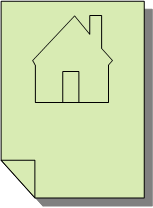
\includegraphics[width=0.25\textwidth]{figures/Homepage-icon.png}
  \end{center}
  \caption{Homepage icon}
  \label{fig:homepageicon}
\end{figure}

\begin{table}[!ht]
  \begin{center}
    \caption{Configurations tested}
    \label{tab:configstested}
    \resizebox{\columnwidth}{!}{%
    \begin{tabular}{l|c} % <-- Alignments: 1st column left, 2nd middle and 3rd right, with vertical lines in between
      \textbf{Configuration} & \textbf{Description} \\
      \hline
      1 & Simple test with one server\\
      2 & Simple test with one server\\
    \end{tabular}
    }
  \end{center}
\end{table}
\sweExpl{Testade konfigurationer}

\section{Implementation …/Modeling/Simulation/…}
\label{sec:implementationDetails}
\sweExpl{Implementering … / modellering / simulering / …}

Two commonly used simulators are:
\begin{description}[labelwidth =\widthof{\textbf{ns-2 or ns-3 simulator}}, leftmargin = !]
    \item[\textbf{Mininet}] This simulator uses traffic control (\texttt{tc}) to simulate network devices connected by links with specific bandwidth, packet loss rates, qdisc methods, etc.
    
    
    \item[\textbf{ns-2 or ns-3 simulator}] These simulators are very useful for simulating wireless communication links between moving devices. You can specify the mobility patterns of the nodes.
\end{description}

\subsection{Some examples of coding}
\engExpl{This section is simply to show some example of how you can include code in your thesis - this is not a section you would have in your thesis.}
\sweExpl{Det här avsnittet är helt enkelt för att visa ett exempel på hur du kan inkludera kod i ditt examensarbete - det här är inte ett avsnitt du skulle ha i ditt examensarbete.}

Listing~\ref{lst:helloWorldInC} shows an example of a simple program written
in C code.

\begin{lstlisting}[language={C}, caption={Hello world in C code}, label=lst:helloWorldInC]
int main() {
printf("hello, world");
return 0;
}
\end{lstlisting}

\engExpl{This template uses the package \texttt{lstlistings} for many different listings. Alternatively, one could use the \texttt{minited} package together with the \texttt{listings} environment, see, for example, \href{https://www.overleaf.com/learn/latex/Code_Highlighting_with_minted}{Code Highlighting with minted}. }

In contrast, Listing~\ref{lst:programmes} is an example of code in Python to
get a list of all of the programs at KTH. Note that on {\DTMsetdatestyle{iso}\DTMdisplaydate{2025}{6}{1}{-1}} the KOPPS API will no longer work.
\engExpl{Note that the change to the iso date format was done in a group so that afterwards the date style returns to what it was, resulting in \DTMdisplaydate{2025}{6}{1}{-1}.}

\lstset{extendedchars=true}  %% This allows character codes in the range 128-255
\begin{lstlisting}[language={Python}, caption={Using a python program to
    access the KTH API to get all of the programs at KTH}, label=lst:programmes]
KOPPSbaseUrl = 'https://www.kth.se'

def v1_get_programmes():
    global Verbose_Flag
    #
    # Use the KOPPS API to get the data
    # note that this returns XML
    url = "{0}/api/kopps/v1/programme".format(KOPPSbaseUrl)
    if Verbose_Flag:
        print("url: " + url)
    #
    r = requests.get(url)
    if Verbose_Flag:
        print("result of getting v1 programme: {}".format(r.text))
    #
    if r.status_code == requests.codes.ok:
        return r.text           # simply return the XML
    #
    return None
\end{lstlisting}
\FloatBarrier

In \Cref{lst:exampleUsingMinted}, line \ref{listinline:ExcelWriter} shows the use of the \texttt{ExcelWriter} function. Line \ref{listinline:UsingToexcel} writes a panda dataframe (named \texttt{comp}) to the spreadsheet, while line \ref{listinline:closingWriter} closes the open spreadsheet.

\begin{listing}[!ht]
\begin{minted}[linenos,breaklines, escapeinside=||]{python}
import pandas as pd
def make_spreadsheet_of_differences(pds):
    global school
    publishers=set()
    writer = pd.ExcelWriter(f'/tmp/{school}_compare_duplicates.xlsx', engine='xlsxwriter') |\label{listinline:ExcelWriter}|
    print("starting")
    for idx, p in enumerate(pds):
        p0=list(p)[0]
        p1=list(p)[1]
        print(f"\nfor {p0} and {p1}")
        comp, publisher1, publisher2=compare_two_records_silent(p0, p1)
        sheet_name=f'{p0}'.split(':')[1]
        print(f'Wrote {sheet_name=}')|\label{listinline:UsingToexcel}|
        comp.to_excel(writer, sheet_name=sheet_name)
        publishers.add(publisher1)
        publishers.add(publisher2)
    
    # Close the Pandas Excel writer and output the Excel file.
    writer.close()|\label{listinline:closingWriter}|
    print(f"{publishers=}")
    return publishers
\end{minted}
\caption{Example of using \texttt{minted} with python code}
\label{lst:exampleUsingMinted}
\end{listing}

\FloatBarrier


\subsection{Some examples of figures in tikz}
\engExpl{This section is simply to show some example of how you can draw your own figures for in your thesis - this is not a section you would have in your thesis.}
\sweExpl{Det här avsnittet är helt enkelt för att visa ett exempel på hur du kan rita dina egna figurer i ditt examensarbete – det här är inte ett avsnitt du skulle ha i ditt examensarbete.}

\Needspace*{5\baselineskip}
These figures are just some examples to show that you can draw your own figures for your thesis. This has two advantages: \first you do not have to worry about copyrights -- as these are your own figures and \Second the text is now readable and not simply a picture of text -- so screen readers can read the figure's contents to someone who is listening to the contents of your thesis.

\subsubsection{Azure's Form Recognizer}
\Cref{fig:processAnInvoice} shows the processing of key-value extraction from a PDF document using Azure's Form Recognizer. 

\tikzset{
    processBox/.style={rectangle, rounded corners, minimum width=3cm, minimum height=1cm,text centered, font=\sffamily, draw=black, fill=red!20},
    largeBox/.style={rectangle, rounded corners, minimum width=3cm, minimum height=4cm,text centered, draw=black}
}
\begin{figure}[!ht]
\resizebox{1.1\textwidth}{!}{%
\begin{tikzpicture}
[align=left,node distance=2cm]

\node (document) [tape,tape bend top=none,draw,font=\sffamily] {PDF\\Document};
\node (GDM) [processBox,  right=0.5cm of document] {OCR};
\node (OCRoutput) [largeBox, right=1cm of GDM] {OCR output};

\node (kvp) [tape,tape bend top=none,draw,font=\sffamily, below=0.25cm of OCRoutput.north] {key-value\\pairs};
\node (entities) [tape,tape bend top=none,draw,font=\sffamily, above=0.35cm of OCRoutput.south] {Entities};
\node (Manual) [processBox, right=1cm of kvp] {Analyze the extracted\\key-value pairs};
\draw [-latex](document) --  (GDM);
\draw [-latex](kvp) --  (Manual);
\path[ draw
     , -latex'] let \p1=(GDM.east), \p2=(kvp.west) in (GDM.east) -- +(0.25*\x2-0.25*\x1, \y1) -- +(0.5*\x2-0.5*\x1, \y2) -- (kvp.west);
\path[ draw
     , -latex'] let \p1=(GDM.east), \p2=(kvp.west), \p3=(entities.west) in (GDM.east) --  +(0.25*\x2-0.25*\x1, \y1) -- +(0.5*\x3-0.5*\x1, \y3) -- (entities.west);
\end{tikzpicture}
}
\caption{The processing of key-value extraction from a PDF document using Azure's Form Recognizer}
  \label{fig:processAnInvoice}
\end{figure}
\FloatBarrier
\subsubsection{Hyper-V with Containers}
 \Cref{fig:hyperVcontainers} shows how Hyper-V deals with containers.
 
 \tikzset{
    container/.style={rectangle, rounded corners, minimum width=2cm, minimum height=1cm,text centered, draw=black, fill=blue!20},
    containerization/.style={rectangle, rounded corners, minimum width=13.25cm, minimum height=1cm,text centered, draw=black, fill=blue!20},
    hypervisor/.style={rectangle, rounded corners, minimum width=13.25cm, minimum height=1cm,text centered, draw=black, fill=red!20},
    os/.style={rectangle, rounded corners, minimum width=13.25cm, minimum height=1cm,text centered, draw=black, fill=orange!20},
    guestos/.style={rectangle, rounded corners, minimum width=2cm, minimum height=1cm,text centered, draw=black, fill=orange!40},
    infrastructure/.style={rectangle, rounded corners, minimum width=13.25cm, minimum height=1cm,text centered, draw=black, fill=green!20},
    hos/.style={rectangle, rounded corners, minimum width=6cm, minimum height=1cm,text centered, draw=black, fill=orange!20},
    kernel/.style={rectangle, rounded corners, minimum width=6cm, minimum height=1cm,text centered, draw=black, fill=purple!20},
    services/.style={rectangle, rounded corners, minimum width=3cm, minimum height=1cm,text centered, draw=black, fill=pink!20]}
}

\begin{figure}[ht!]
    \centering
\resizebox{1\textwidth}{!}{%
\begin{tikzpicture}
[align=center,node distance=2cm]

\node (Infrastructure) [infrastructure, text width=13cm, text centered] {Infrastructure};
\node (OS1) [hos, anchor=north west, align=left, above=1.5cm of Infrastructure.north west, anchor=north west, text width=6cm, text centered] {Host OS};

\node (OS2) [hos, anchor= west, align=left, right=0.5cm of OS1.east, text width=6cm, anchor= west, text centered] {Host OS};

\node (Kernel1) [kernel, anchor=north west, align=left, above=1.5cm of OS1.north east, anchor=north east, text width=3cm, text centered] {Kernel};

\node (Kernel2) [kernel, anchor=north west, align=left, above=1.5cm of OS2.north east, anchor=north east, text width=3cm, text centered] {Kernel};

\node (ServiceA) [container, anchor=east, above=1 cm of Kernel1.east, anchor=east] {Services};
\node (AppA) [container,  left=0.25cm of ServiceA] {App 1};

\node (ServiceB) [container, anchor=east, above=1 cm of Kernel2.east, anchor=east] {Services};
\node (AppB) [container,  left=0.25cm of ServiceB] {App 2};
%\node (AppC) [container,  right=0.25cm of AppB] {App 3};

\draw[black,thick,dashed] ($(OS2.north west)+(-0.3,3.75)$)  rectangle ($(OS2.south east)+(0.5,-0.3)$);
\node[text width=5cm, text=red, above=0.1cm of ServiceB] 
    {\textbf{Container}};

\draw[red,thick,dotted] ($(Kernel2.north west)+(-0.3,1.6)$)  rectangle ($(Kernel2.south east)+(0.3,-0.3)$);
\node[text width=5cm, text=black, above=0.8cm of ServiceB] 
    {\textbf{VM}};
\end{tikzpicture}
}
    \caption{Hyper-V with containers}
    \label{fig:hyperVcontainers}
\end{figure}
\FloatBarrier
\subsubsection{\glsfmtshort{VM} versus Containers}
\Cref{fg:vmsVersusContainers} shows a comparison of virtual machines (VMs) versus containers.

\begin{figure*}[ht!]
    \centering
    \begin{subfigure}[t]{0.5\textwidth}
        \centering
\resizebox{1\textwidth}{!}{%
\begin{tikzpicture}
[align=left,node distance=2cm]

\node (AppA) [container,align=left] {App 1};
\node (AppB) [container,  right=0.25cm of AppA] {App 2};
\node (AppC) [container,  right=0.25cm of AppB] {App 3};

\node (GosA) [guestos,align=left,  below=0.25cm of AppA.south west,anchor=north west] {Guest OS};
\node (GosB) [guestos,  right=0.25cm of GosA] {Guest OS};
\node (GosC) [guestos,  right=0.25cm of GosB] {Guest OS};

\draw [decoration={brace,amplitude=0.5em},decorate, ultra thick,gray, transform canvas={xshift = 0.5cm}]
       (AppC.north -| AppC.east) -- (GosC.south -| AppC.east);
\node[text width=5cm,  right=1cm of GosC.north east] 
    {\textbf{VMs}};

\node (Hypervisor) [hypervisor, anchor=north west, align=left, below=0.25cm of GosA.south west, anchor=north west, text width=13cm, text centered] {Hypervisor};

\node (OS) [os, anchor=north west, align=left, below=0.25cm of Hypervisor.south west, anchor=north west, text width=13cm, text centered] {Host OS};

\node (Infrastructure) [infrastructure, anchor=north west, align=left, below=0.25cm of OS.south west, anchor=north west, text width=13cm, text centered] {Infrastructure};


\end{tikzpicture}
}
        \caption{VM}
    \end{subfigure}%
    ~ 
    \begin{subfigure}[t]{0.5\textwidth}
        \centering
        \resizebox{1\textwidth}{!}{%
\begin{tikzpicture}
[align=left,node distance=2cm]

\node (AppA) [container,align=left] {App 1};
\node (AppB) [container,  right=0.25cm of AppA] {App 2};
\node (AppC) [container,  right=0.25cm of AppB] {App 3};
\node[text width=5cm,  right=0.25cm of AppC] 
    {\textbf{Apps running in Containers}};


\node (Containerization) [containerization, anchor=north west, align=left, below=0.25cm of AppA.south west, anchor=north west, text width=13cm, text centered] {Docker Engine};

\node (OS) [os, anchor=north west, align=left, below=0.25cm of Containerization.south west, anchor=north west, text width=13cm, text centered] {Host OS};

\node (Infrastructure) [infrastructure, anchor=north west, align=left, below=0.25cm of OS.south west, anchor=north west, text width=13cm, text centered] {Infrastructure};


\end{tikzpicture}
}
        \caption{Containers}
    \end{subfigure}
    \caption{Virtual machines (VMs) versus Containers}
    \label{fg:vmsVersusContainers}
\end{figure*}

\cleardoublepage
\chapter{Results and Analysis}
\label{ch:resultsAndAnalysis}
\sweExpl{svensk: Resultat och Analys}

\engExpl{Sometimes this is split into two chapters.\\Keep in mind: How you are going to evaluate what you have done? What are your metrics?\\Analysis of your data and proposed solution\\Does this meet the goals which you had when you started?}

In this chapter, we present the results and discuss them.

\sweExpl{I detta kapitel presenterar vi resultaten och diskutera dem.\\Ibland delas detta upp i två kapitel.\\Hur du ska utvärdera vad du har gjort? Vad är din statistik?\\Analys av data och föreslagen lösning\\Innebär detta att uppfyllelse av de mål som du hade när du började?}

\section{Major results}
\sweExpl{Huvudsakliga resultat}

Some statistics of the delay measurements are shown in Table~\ref{tab:delayMeasurements}.
The delay has been computed from the time the GET request is received until the response is sent.

\sweExpl{Lite statistik av fördröjningsmätningarna visas i Tabell~\ref{tab:delayMeasurements}. Förseningen har beräknats från den tidpunkt då begäran GET tas emot fram till svaret skickas.}

\begin{table}[!ht]
  \begin{center}
    \caption{Delay measurement statistics}
    \label{tab:delayMeasurements}
    \begin{tabular}{l|S[table-format=4.2]|S[table-format=3.2]} % <-- Alignments: 1st column left, 2nd middle and 3rd right, with vertical lines in between
      \textbf{Configuration} & \textbf{Average delay (ns)} & \textbf{Median delay (ns)}\\
      \hline
      1 & 467.35 & 450.10\\
      2 & 1687.5 & 901.23\\
    \end{tabular}
  \end{center}
\end{table}

Table \ref{tab:ping_results} shows the measurement of round trip times from four hosts to and from a server.
\begin{table}[ht!]
\caption[RTT for 4 hosts]{Result for the ping measurements of RTT for 4 hosts} 
\label{tab:ping_results}
\vspace{1em}
\centering
\begin{tabular}{l *{4}{S[table-format=2.3]}}
{} & \multicolumn{4}{c}{host to server RTT in ms} \\
\cmidrule{2-5}
Host & \multicolumn{1}{c}{min}  & \multicolumn{1}{c}{avg} & \multicolumn{1}{c}{max} & \multicolumn{1}{c}{mdev} \\
\midrule
h1 & 5.625 & 5.625 & 5.625 & 0.0 \\
h2 & 2.909 & 2.909 & 1.909 & 0.0 \\
h3 & 5.007 & 5.007 & 5.007 & 0.0 \\
h4 & 2.308 & 2.308 & 2.308 & 0.0 \\
\midrule
\end{tabular}
\end{table}
\FloatBarrier

\sweExpl{Fördröj mätstatistik}
\sweExpl{Konfiguration | Genomsnittlig fördröjning (ns) | Median fördröjning (ns)}

Figure \ref{fig:processing_vs_payload_length} shows an example of the performance as measured in the experiments.

\begin{figure}[!ht]
% GNUPLOT: LaTeX picture
\setlength{\unitlength}{0.240900pt}
\ifx\plotpoint\undefined\newsavebox{\plotpoint}\fi
\begin{picture}(1500,900)(0,0)
\sbox{\plotpoint}{\rule[-0.200pt]{0.400pt}{0.400pt}}%
\put(171.0,131.0){\rule[-0.200pt]{4.818pt}{0.400pt}}
\put(151,131){\makebox(0,0)[r]{ 1.5}}
\put(1419.0,131.0){\rule[-0.200pt]{4.818pt}{0.400pt}}
\put(171.0,212.0){\rule[-0.200pt]{4.818pt}{0.400pt}}
\put(151,212){\makebox(0,0)[r]{ 2}}
\put(1419.0,212.0){\rule[-0.200pt]{4.818pt}{0.400pt}}
\put(171.0,292.0){\rule[-0.200pt]{4.818pt}{0.400pt}}
\put(151,292){\makebox(0,0)[r]{ 2.5}}
\put(1419.0,292.0){\rule[-0.200pt]{4.818pt}{0.400pt}}
\put(171.0,373.0){\rule[-0.200pt]{4.818pt}{0.400pt}}
\put(151,373){\makebox(0,0)[r]{ 3}}
\put(1419.0,373.0){\rule[-0.200pt]{4.818pt}{0.400pt}}
\put(171.0,454.0){\rule[-0.200pt]{4.818pt}{0.400pt}}
\put(151,454){\makebox(0,0)[r]{ 3.5}}
\put(1419.0,454.0){\rule[-0.200pt]{4.818pt}{0.400pt}}
\put(171.0,534.0){\rule[-0.200pt]{4.818pt}{0.400pt}}
\put(151,534){\makebox(0,0)[r]{ 4}}
\put(1419.0,534.0){\rule[-0.200pt]{4.818pt}{0.400pt}}
\put(171.0,615.0){\rule[-0.200pt]{4.818pt}{0.400pt}}
\put(151,615){\makebox(0,0)[r]{ 4.5}}
\put(1419.0,615.0){\rule[-0.200pt]{4.818pt}{0.400pt}}
\put(171.0,695.0){\rule[-0.200pt]{4.818pt}{0.400pt}}
\put(151,695){\makebox(0,0)[r]{ 5}}
\put(1419.0,695.0){\rule[-0.200pt]{4.818pt}{0.400pt}}
\put(171.0,776.0){\rule[-0.200pt]{4.818pt}{0.400pt}}
\put(151,776){\makebox(0,0)[r]{ 5.5}}
\put(1419.0,776.0){\rule[-0.200pt]{4.818pt}{0.400pt}}
\put(171.0,131.0){\rule[-0.200pt]{0.400pt}{4.818pt}}
\put(171,90){\makebox(0,0){ 0}}
\put(171.0,756.0){\rule[-0.200pt]{0.400pt}{4.818pt}}
\put(298.0,131.0){\rule[-0.200pt]{0.400pt}{4.818pt}}
\put(298,90){\makebox(0,0){ 10}}
\put(298.0,756.0){\rule[-0.200pt]{0.400pt}{4.818pt}}
\put(425.0,131.0){\rule[-0.200pt]{0.400pt}{4.818pt}}
\put(425,90){\makebox(0,0){ 20}}
\put(425.0,756.0){\rule[-0.200pt]{0.400pt}{4.818pt}}
\put(551.0,131.0){\rule[-0.200pt]{0.400pt}{4.818pt}}
\put(551,90){\makebox(0,0){ 30}}
\put(551.0,756.0){\rule[-0.200pt]{0.400pt}{4.818pt}}
\put(678.0,131.0){\rule[-0.200pt]{0.400pt}{4.818pt}}
\put(678,90){\makebox(0,0){ 40}}
\put(678.0,756.0){\rule[-0.200pt]{0.400pt}{4.818pt}}
\put(805.0,131.0){\rule[-0.200pt]{0.400pt}{4.818pt}}
\put(805,90){\makebox(0,0){ 50}}
\put(805.0,756.0){\rule[-0.200pt]{0.400pt}{4.818pt}}
\put(932.0,131.0){\rule[-0.200pt]{0.400pt}{4.818pt}}
\put(932,90){\makebox(0,0){ 60}}
\put(932.0,756.0){\rule[-0.200pt]{0.400pt}{4.818pt}}
\put(1059.0,131.0){\rule[-0.200pt]{0.400pt}{4.818pt}}
\put(1059,90){\makebox(0,0){ 70}}
\put(1059.0,756.0){\rule[-0.200pt]{0.400pt}{4.818pt}}
\put(1185.0,131.0){\rule[-0.200pt]{0.400pt}{4.818pt}}
\put(1185,90){\makebox(0,0){ 80}}
\put(1185.0,756.0){\rule[-0.200pt]{0.400pt}{4.818pt}}
\put(1312.0,131.0){\rule[-0.200pt]{0.400pt}{4.818pt}}
\put(1312,90){\makebox(0,0){ 90}}
\put(1312.0,756.0){\rule[-0.200pt]{0.400pt}{4.818pt}}
\put(1439.0,131.0){\rule[-0.200pt]{0.400pt}{4.818pt}}
\put(1439,90){\makebox(0,0){ 100}}
\put(1439.0,756.0){\rule[-0.200pt]{0.400pt}{4.818pt}}
\put(171.0,131.0){\rule[-0.200pt]{0.400pt}{155.380pt}}
\put(171.0,131.0){\rule[-0.200pt]{305.461pt}{0.400pt}}
\put(1439.0,131.0){\rule[-0.200pt]{0.400pt}{155.380pt}}
\put(171.0,776.0){\rule[-0.200pt]{305.461pt}{0.400pt}}
\put(30,453){\rotatebox{-270}{\makebox(0,0){Processing time (ms)}}}
\put(805,29){\makebox(0,0){Payload size (bytes)}}
\put(868.0,131.0){\rule[-0.200pt]{0.400pt}{84.074pt}}
\put(995.0,131.0){\rule[-0.200pt]{0.400pt}{98.287pt}}
\put(1173.0,131.0){\rule[-0.200pt]{0.400pt}{118.041pt}}
\put(1325.0,131.0){\rule[-0.200pt]{0.400pt}{134.904pt}}
\put(1350.0,131.0){\rule[-0.200pt]{0.400pt}{137.795pt}}
\put(1439.0,131.0){\rule[-0.200pt]{0.400pt}{155.380pt}}
\end{picture}
\caption[A GNUplot figure]{Processing time vs. payload length}\vspace{0.5cm}
\label{fig:processing_vs_payload_length}
\end{figure}
\FloatBarrier		

Given these measurements, we can calculate our processing bit rate as the inverse of the time it takes to process an additional byte divided by 8 bits per byte:

\[
	\text{bit rate} = \frac{1}{\frac{\text{time}_{\text{byte}}}{8}} = 20.03 \quad kb/s
\] 

\Cref{tab:majorMarkupLMDetailedResult} shows another table in which some values have been set in bold (using \textbackslash B) to emphasize them. Note how the \texttt{S} formatting has been modified so that it considers the weight of the characters and this is able to decimal align even these hold-faced numbers with the numbers in the column above them.

\begin{table}[!ht]
    \centering
    \caption{Median values of sandwich attributes}
    \label{tab:majorMarkupLMDetailedResult}
    \begin{tabular}{l *{2}{S[detect-weight,mode=text,table-format=3.2]}}
        & \multicolumn{2}{c}{\textbf{sites}}\\
        \cmidrule{2-3}
        \textbf{Attribute} & \textbf{A} & \textbf{B} \\
        \midrule
        price (in SEK) & 36.5 & 71.3 \\
        protean (g) & 97.2 & 100.0 \\
        salt (mg) & 9.7 & 9.3 \\
        \hline
        \textbf{Average customer rating in \%} & \B 82.2 & \B 89.9 \\
        \midrule
    \end{tabular}
\end{table}
\FloatBarrier


\Needspace*{4\baselineskip}
\Cref{fig:stackedrust} shows a stacked bar chart using pgfplots. It illustrates how easy it is to take a set of data and make a stacked bar plot. One of the features is the shifted values -- this is very useful when the bar itself is too small to put the value into.

\pgfplotstableread{
Label Numbers  Refs  Struct/Enum  Heap  Arrays
cratesio 70.04 19.83 8.31 1.3 0.52
librs 49.26 30.49 10.80 7.92 1.53
rustc 55.01 24.80 11.54 6.16 2.49
}\testdata


\pgfkeys{
    /pgf/number format/.cd,
    fixed,
    fixed zerofill,
    precision=2
}
\begin{figure}[ht!]
    \centering
    \scalebox{0.9}{
    \begin{tikzpicture}
    \begin{axis}[
        ybar stacked,
        %reverse legend,
        reverse legend=false,
        %https://tex.stackexchange.com/questions/88892/pgfplots-bar-plot-spacing-inbetween-bars
        enlarge x limits=0.4,
	    bar width=45pt,
        /pgfplots/nodes near coords*/.append style={
        every node near coord/.style={
            color=black,
            font=\small,
            name=X,
%            shift={    
%                (50pt,25pt)
%                },
            xshift={50pt},
                yshift ={
                ifthenelse((\plotnum == 4), 30pt,20pt)},
            },
            scatter/@post marker code/.append code={
                \node(Y){};
                \draw(X)--(Y.center);
            }
        },
	    nodes near coords,
        bar shift=5pt,
        ymin=0,
        ymax=115,
        xtick=data,
        width=1\textwidth,
        legend style={draw=none},
        legend image post style={scale=2.0},
        legend style={
            at={(0.5,-0.2)},
            anchor=north,
            legend columns=-2,
            font=\large,
            %mark size=20pt,
        },
        ylabel=Percentage points (\%),
        xticklabels from table={\testdata}{Label},
        xticklabel style={rotate=30},
    ]
    \addplot  table [y=Numbers, meta=Label, x expr=\coordindex] {\testdata};
    \addlegendentry{Numbers}
    \addplot table [y=Refs, meta=Label, x expr=\coordindex] {\testdata};
    \addlegendentry{Refs}
    \addplot  table [y=Struct/Enum, meta=Label, x expr=\coordindex] {\testdata};
    \addlegendentry{Struct/Enum}
    \addplot  table [y=Heap, meta=Label, x expr=\coordindex] {\testdata};
    \addlegendentry{Heap}
    \addplot  table [y=Arrays, meta=Label, x expr=\coordindex] {\testdata};
    \addlegendentry{Arrays}
    \end{axis}
    \end{tikzpicture}}
\caption{Rust types distribution for the compiler, crates.io, and lib.rs.
(percentage) - appears here with the permission of the author - see the thesis at \url{https://urn.kb.se/resolve?urn=urn\%3Anbn\%3Ase\%3Akth\%3Adiva-332124}}
\label{fig:stackedrust}
\end{figure}
\FloatBarrier



\section{Reliability Analysis}
\sweExpl{Analys av tillförlitlighet\\
Tillförlitlighet i metod och data}

\section{Validity Analysis}
\sweExpl{Analys av validitet\\
Validitet i metod och data}

\cleardoublepage
\chapter{Discussion}
\label{ch:discussion}
\sweExpl{Diskussion\\
Förbättringsförslag?}
\generalExpl{This can be a separate chapter or a section in the previous chapter.}

\cleardoublepage
\chapter{Conclusions and Future work}
\label{ch:conclusionsAndFutureWork}
\sweExpl{Slutsats och framtida arbete}

\generalExpl{Add text to introduce the subsections of this chapter.}

\section{Conclusions}
\label{sec:conclusions}
\sweExpl{Slutsatser}
\engExpl{Describe the conclusions (reflect on the whole introduction given in Chapter 1).}


  
\engExpl{Discuss the positive effects and the drawbacks.\\
Describe the evaluation of the results of the degree project.\\
Did you meet your goals?\\
What insights have you gained?\\
What suggestions can you give to others working in this area?\\
If you had it to do again, what would you have done differently?}

\sweExpl{Uppfyllde du dina mål?\\
Vilka insikter har du fått?\\
Vilka förslag kan du ge till andra som arbetar inom detta område?
Om du skulle göra detta igen, vad skulle du ha gjort annorlunda?}

\section{Limitations}
\label{sec:limitations}
\sweExpl{Begränsande faktorer\\Vad gjorde du som begränsade dina ansträngningar? Vilka är begränsningarna i dina resultat?}
\engExpl{What did you find that limited your efforts? What are the limitations of your results?}


\section{Future work}
\label{sec:futureWork}
\sweExpl{Vad du har kvar ogjort?\\Vad är nästa självklara saker som ska göras?\\Vad tips kan du ge till nästa person som kommer att följa upp på ditt arbete?}
\engExpl{Describe valid future work that you or someone else could or should do.\\
Consider: What you have left undone? What are the next obvious things to be done? What hints can you give to the next person who is going to follow up on your work?}



Due to the breadth of the problem, only some of the initial goals have been
met. In these section we will focus on some of the remaining issues that
should be addressed in future work. ...

\subsection{What has been left undone?}
\label{what-has-been-left-undone}

The prototype does not address the third requirment, \ie a yearly unavailability of less than 3 minutes; this remains an open problem. ...

\subsubsection{Cost analysis}
\generalExpl{Example of a missing component}
The current prototype works, but the performance from a cost perspective makes this an impractical solution. Future work must reduce the cost of this solution; to do so, a cost analysis needs to first be done. ...

\subsubsection{Security}
\generalExpl{Example of a missing component}
A future research effort is needed to address the security holes that results from using a self-signed certificate. Page filling text mass. Page filling text mass. ...


\subsection{Next obvious things to be done}

In particular, the author of this thesis wishes to point out xxxxxx remains as a problem to be solved. Solving this problem is the next thing that should be done. ...

\section{Reflections}
\label{sec:reflections}
\sweExpl{Reflektioner}
\sweExpl{Vilka är de relevanta ekonomiska, sociala, miljömässiga och etiska aspekter av ditt arbete?}
\engExpl{What are the relevant economic, social,
  environmental, and ethical aspects of your work?
}



One of the most important results is the reduction in the amount of
energy required to process each packet while at the same time reducing the
time required to process each packet.

The thesis contributes to the \gls{UN}\enspace\glspl{SDG} numbers 1 and 9 by
xxxx. 




\noindent\rule{\textwidth}{0.4mm}
\engExpl{In the references, let Zotero or other tool fill this in for you. I suggest an extended version of the IEEE style, to include URLs, DOIs, ISBNs, etc., to make it easier for your reader to find them. This will make life easier for your opponents and examiner. \\IEEE Editorial Style Manual: \url{https://www.ieee.org/content/dam/ieee-org/ieee/web/org/conferences/style_references_manual.pdf}}
\sweExpl{Låt Zotero eller annat verktyg fylla i det här för dig. Jag föreslår en utökad version av IEEE stil - att inkludera webbadresser, DOI, ISBN osv. - för att göra det lättare för läsaren att hitta dem. Detta kommer att göra livet lättare för dina opponenter och examinator.}

\cleardoublepage
% Print the bibliography (and make it appear in the table of contents)
\renewcommand{\bibname}{References}


\iftoggle{biblatex}{
    %\typeout{Biblatex current language is \currentlang}
    \printbibliography[heading=bibintoc]
}{
    \phantomsection  % make it include a hyperref - see https://tex.stackexchange.com/a/98995
    \addcontentsline{toc}{chapter}{References}
    \bibliography{references}
}



\warningExpl{If you do not have an appendix, do not include the \textbackslash cleardoublepage command below; otherwise, the last page number in the metadata will be one too large.}
\cleardoublepage
\appendix
\renewcommand{\chaptermark}[1]{\markboth{Appendix \thechapter\relax:\thinspace\relax#1}{}}
\chapter{Supporting materials}
\label{sec:supportingMaterial}
\generalExpl{Here is a place to add supporting material that can help others build upon your work. You can include files as attachments to the PDF file or indirectly via URLs. Alternatively, consider adding supporting material uploaded as separate files in DiVA.}

% Attach the BibTeX for your references to make it easy for a reader to find and use them
The BibTeX references used in this thesis are attached. \attachfile[description={references.bib}]{references.bib}

% Attach source code file(s) or add a URL to the github or other repository
Some source code relevant to this project can be found at \url{https://github.com/gqmaguirejr/E-learning} and \url{https://github.com/gqmaguirejr/Canvas-tools}.

Your reader can access the attached (embedded) files using a PDF tool such as Adobe Acrobat Reader using the paperclip icon in the left menu, as shown in \Cref{fig:PDFreaderPaperclipExample} or by right-clicking on the push-pin icon in the PDF file and then using the menu to save the embedded file as shown in \Cref{fig:PDFreaderPushpinExample}.

An argument for including supporting material in the PDF file is that it will be available to anyone who has a copy of the PDF file. As a result, they do not have to look elsewhere for this material. This comes at the cost of a larger PDF file. However, the embedded files are encoded into a compressed stream within the PDF file; thus, reducing the number of additional bytes. For example, the references.bib file that was used in this example is \SI{10617}{\byte} in size but only occupies \SI{4261}{\byte} in the PDF file.

\warningExpl{DiVA is limited to $\approx$\SI{1}{\giga\byte} for each supporting file. If you have very large amounts of supporting material, you will probably want to use one of the data repositories. For additional help with this, contact KTH Library via 
\href{mailto:researchdata@kth.se}{researchdata@kth.se}.\\As of Spring 2024, there are plans to migrate this supporting data from DiVA to a research data repository.
}

\begin{figure}[!ht]
  \begin{center}
    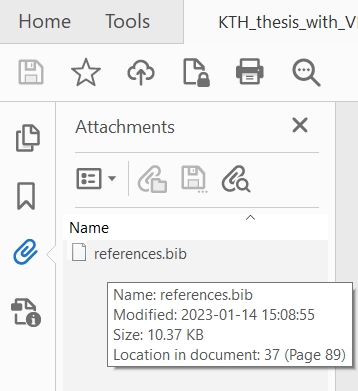
\includegraphics[width=0.50\textwidth]{README_notes/pdf-viewer-attached-files.png}
  \end{center}
  \caption{Adobe Acrobat Reader using the paperclip icon for the attached references.bib file}
  \label{fig:PDFreaderPaperclipExample}
\end{figure}
\FloatBarrier

\begin{figure}[!ht]
  \begin{center}
    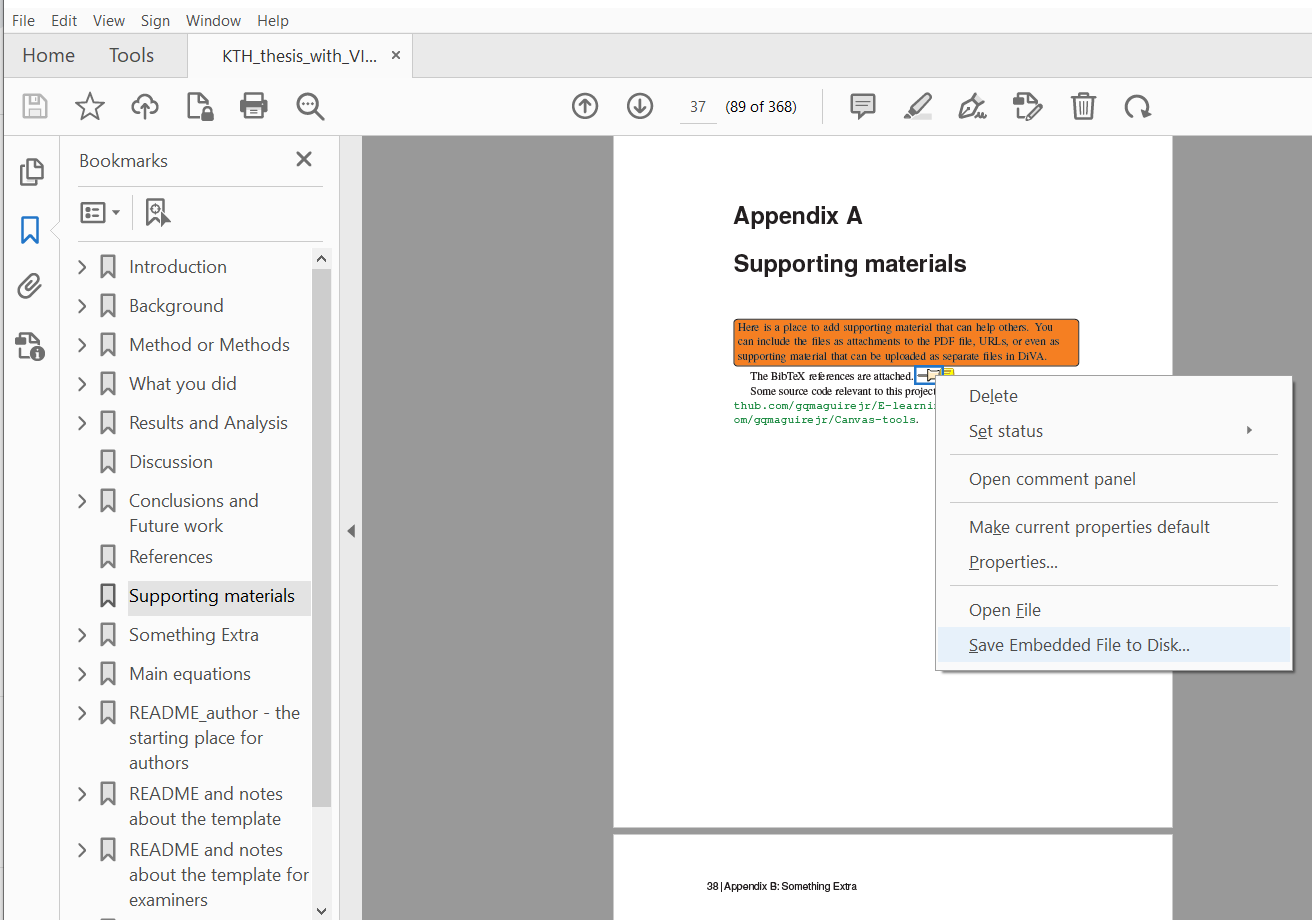
\includegraphics[width=0.99\textwidth]{README_notes/Bib-save-embedded-example.png}
  \end{center}
  \caption{Adobe Acrobat Reader after right-clicking on the push-pin icon for the attached references.bib file}
  \label{fig:PDFreaderPushpinExample}
\end{figure}
\FloatBarrier
\cleardoublepage

\chapter{Something Extra}
\sweExpl{svensk: Extra Material som Bilaga}

\section{Just for testing KTH colors}
\iftoggle{digitaloutput}{
    \textbf{You have selected to optimize for digital output}
}{
    \textbf{You have selected to optimize for print output}
}

\begin{itemize}[noitemsep]
    \item Primary color
    \begin{itemize}
    \item \textcolor{kth-blue}{kth-blue \iftoggle{digitaloutput}{
    actually Deep sea
    }{}} {\color{kth-blue} \rule{0.3\linewidth}{1mm} }\\

    \item \textcolor{kth-blue80}{kth-blue80} {\color{kth-blue80} \rule{0.3\linewidth}{1mm} }\\
\end{itemize}

\item  Secondary colors
\begin{itemize}[noitemsep]
    \item \textcolor{kth-lightblue}{kth-lightblue \iftoggle{digitaloutput}{
    actually Stratosphere
    }{}} {\color{kth-lightblue} \rule{0.3\linewidth}{1mm} }\\

    \item \textcolor{kth-lightred}{kth-lightred \iftoggle{digitaloutput}{
    actually Fluorescence}{}} {\color{kth-lightred} \rule{0.3\linewidth}{1mm} }\\

    \item \textcolor{kth-lightred80}{kth-lightred80} {\color{kth-lightred80} \rule{0.3\linewidth}{1mm} }\\

    \item \textcolor{kth-lightgreen}{kth-lightgreen \iftoggle{digitaloutput}{
    actually Front-lawn}{}} {\color{kth-lightgreen} \rule{0.3\linewidth}{1mm} }\\

    \item \textcolor{kth-coolgray}{kth-coolgray \iftoggle{digitaloutput}{
    actually Office}{}} {\color{kth-coolgray} \rule{0.3\linewidth}{1mm} }\\

    \item \textcolor{kth-coolgray80}{kth-coolgray80} {\color{kth-coolgray80} \rule{0.3\linewidth}{1mm} }
\end{itemize}
\end{itemize}

\textcolor{black}{black} {\color{black} \rule{\linewidth}{1mm} }

% Include an example of using nomenclature
\ifnomenclature
    \cleardoublepage
    \chapter{Main equations}
    \label{ch:NomenclatureExamples}
    This appendix gives some examples of equations that are used throughout this thesis.
    \section{A simple example}
    The following example is adapted from Figure 1 of the documentation for the package nomencl (\url{https://ctan.org/pkg/nomencl}).
    \begin{equation}\label{eq:mainEq}
    a=\frac{N}{A}
    \end{equation}
    \nomenclature{$a$}{The number of angels per unit area\nomrefeq}%       %% include the equation number in the list
    \nomenclature{$N$}{The number of angels per needle point\nomrefpage}%  %% include the page number in the list
    \nomenclature{$A$}{The area of the needle point}%
    The equation $\sigma = m a$%
    \nomenclature{$\sigma$}{The total mass of angels per unit area\nomrefeqpage}%
    \nomenclature{$m$}{The mass of one angel}
follows easily from \Cref{eq:mainEq}.

    \section{An even simpler example}
    The formula for the diameter of a circle is shown in \Cref{eq:secondEq} area of a circle in \cref{eq:thirdEq}.
    \begin{equation}\label{eq:secondEq}
    D_{circle}=2\pi r
    \end{equation}
    \nomenclature{$D_{circle}$}{The diameter of a circle\nomrefeqpage}%
    \nomenclature{$r$}{The radius of a circle\nomrefeqpage}%

    \begin{equation}\label{eq:thirdEq}
    A_{circle}=\pi r^2
    \end{equation}
    \nomenclature{$A_{circle}$}{The area of a circle\nomrefeqpage}%

    Some more text that refers to \eqref{eq:thirdEq}.
\fi  %% end of nomenclature example

\cleardoublepage
% ---------------------------------------------------------------------------
% Template documentation (README_author / README_notes) is disabled here so
% pdflatex exits cleanly: those files expect extra glossary types and Unicode
% glyphs that break pdfLaTeX and stop latexmk before BibTeX finishes---which
% leaves all citations as [?]. Re-enable only when you need to edit the KTH
% template itself (prefer XeLaTeX/LuaLaTeX and the full README glossary setup).
% ---------------------------------------------------------------------------
%\include{README_author}
%\subfile{README_author}
%
%\cleardoublepage
%\input{README_notes/README_notes}

\begin{comment}
% If you actually want to have the full table of National Subject Categories (temporarily) include this appendix
\subfile{README_notes/National_Subject_Categories}
\cleardoublepage
\end{comment}

\begin{comment}
% Information for examiners
\ifxeorlua
\cleardoublepage
\input{README_notes/README_examiner_notes}
\fi
\end{comment}

\begin{comment}
% Information for administrators
\ifxeorlua
\cleardoublepage
\input{README_notes/README_for_administrators.tex}
\fi
\end{comment}

\begin{comment}
% Information for Course Coordinators
\ifxeorlua
\cleardoublepage
\input{README_notes/README_for_course_coordinators}
\fi
\end{comment}

%% The following label is necessary for computing the last page number of the body of the report to include in the "For DIVA" information
\label{pg:lastPageofMainmatter}

\cleardoublepage
\clearpage\thispagestyle{empty}\mbox{} % empty page with backcover on the other side
\kthbackcover
\fancyhead{}  % Do not use header on this extra page or pages
\section*{€€€€ For DIVA €€€€}
\lstset{numbers=none} %% remove any list line numbering
\divainfo{pg:lastPageofPreface}{pg:lastPageofMainmatter}

% If there is an acronyms.tex file,
% add it to the end of the For DIVA information
% so that it can be used with the abstracts
% Note that the option "nolol" stops it from being listed in the List of Listings

% The following bit of ugliness is because of the problems PDFLaTeX has handling a non-breaking hyphen
% unless it is converted to UTF-8 encoding.
% If you do not use such characters in your acronyms, this could be simplified.
\ifxeorlua
\IfFileExists{lib/acronyms.tex}{
\section*{acronyms.tex}
\lstinputlisting[language={[LaTeX]TeX}, nolol, basicstyle=\ttfamily\color{black},
commentstyle=\color{black}, backgroundcolor=\color{white}]{lib/acronyms.tex}
}
{}
\else
\IfFileExists{lib/acronyms-for-pdflatex.tex}{
\section*{acronyms.tex}
\lstinputlisting[language={[LaTeX]TeX}, nolol, basicstyle=\ttfamily\color{black},
commentstyle=\color{black}, backgroundcolor=\color{white}]{lib/acronyms-for-pdflatex.tex}
}
{}
\fi


\end{document}
